\documentclass{article}
\usepackage{graphicx}
\usepackage{float}
\usepackage{titlesec}
\usepackage{datetime}
\usepackage{geometry}
\usepackage{placeins}
\usepackage{minted}
\usepackage{xcolor}
\usepackage{listings}
\usepackage{caption}
\usepackage[document]{ragged2e}
\usepackage[hidelinks]{hyperref}
\usepackage{enumitem}
\usepackage{booktabs}
\geometry{
 a4paper,
 left=25mm,
 top=25mm,
 }
\captionsetup{hypcap=false} 
\newdateformat{daymonthyear}{\THEDAY .\THEMONTH .\THEYEAR}
\title{
  \centering
  
\includegraphics[width=\textwidth]{src/images/logo_PWr_kolor_poziom.png}\\
  \fontsize{28pt}{30pt}\selectfont Programowanie efektywnych algorytmów\\
  \fontsize{14pt}{30pt}\selectfont Problem komiwojażera (TSP)}
\author{Krzysztof Zalewa}
\date{\daymonthyear\today}
\renewcommand*\contentsname{Spis treści}
\renewcommand{\figurename}{Rysunek}
\renewcommand{\listingscaption}{Fragment kodu}
\begin{document}
    \maketitle
    \pagebreak
    \tableofcontents
    \FloatBarrier
    \raggedright
    \section{Specyfikacja sprzętu użytego do badań}
      Badania zostały wykonanie na komputerze stacjonarnym o specyfikacji: \linebreak
      \textbf{Procesor:} Intel(R) Core(TM) i7-9700K CPU \linebreak
      \textbf{Zegar:} 3.60GHz \linebreak
      \textbf{Wielkość pamięci RAM:} 32,0 GB (dostępne: 31,8 GB) \linebreak
      \begin{figure}[ht]
        \centering
        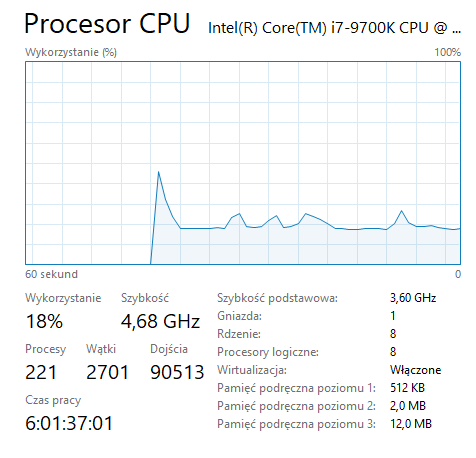
\includegraphics[width=\textwidth]{src/images/Zurzycie_procesora_Tabu.png}
        \caption{Zurzycie procesora w trakcie wykonywania algorytmu Tabu search}
        \label{fig:procTabu}
      \end{figure}
      \FloatBarrier
      
    \section{Instancje użyte w badaniach}
      Do badań użyłem macierzy z \hyperref[src:TspLib]{TspLib[~\ref*{src:TspLib}]} \linebreak
      \textbf{Macierze symetryczne} - rat99.tsp,pr152.tsp,ts225.tsp oraz pr264.tsp \linebreak
      \textbf{Macierze asymetryczne} - ftv33.atsp,ftv64.atsp,\hyperref[txt:explanation1]{kro124p.atsp*}  oraz ftv170.atsp \linebreak
      Gdzie najleprze znane rozwiązania to :
      \begin{table} 
        \centering
        \begin{tabular}{|r|r|r|r|r|r|r|r|r|}
          \hline
          &\multicolumn{4}{|c|}{Symetryczne} & \multicolumn{4}{|c|}{Asymetryczne} \\ \hline\
          Instancje & rat99 & pr152 & ts225 & pr264 & ftv33 & ftv64 & \hyperref[txt:explanation1]{kro124p*}  & ftv170 \\ \hline
          & 1211 & 73682 & 126643 & 49135 & 1286 & 1839 & 36230 & 2755 \\ \hline
        \end{tabular}
        \caption{Optymalne wyniki z TspLib}
        \label{txt:opt}
      \end{table}
      \FloatBarrier
      \label{txt:explanation1}
      * Mimo tego że powinna być to instancja o 124 wierzchołkach po konwersji 
      otrzymuję tylko 100 wierzchołków. Pozostałe instancje konwertują się poprawnie.     
    \section{Tabu search}
      \subsection{Opis Algorytmu}
        Algorytm tabu search jest algorytmem metahurystycznym służącym do rozwiązywania
        problemów optymalizacyjnych. Algorytm ten przechowuje część otrzymanych wcześniej 
        rozwiązań w tablicy tabu. Takie podejście sprawia że szansa na ponowne wybranie
        tego samego rozwiązania znacznie maleje. Sprawia to też że jest mniejsza szansa 
        na utknięcie w pętli. Algorytm ten można jeszcze usprawnić poprzez dodanie 
        warunku krytycznego i strategii dywersyfikacji.\linebreak
        \textbf{Warunek krytyczny: } Jeżeli otrzymana wartość jest mniejsza
        od najlepszej do tej pory znalezionej wartości ale ścieżka znajduje się
        w tabu to i tak przypisujemy obecną wartość do najlepszej.\linebreak
        \textbf{Strategia dywersyfikacji: } Jeżeli przez określoną liczbę iteracji algorytmu
        wartość się nie poprawiła zmieniamy wybraną ścieżkę. W mojej implementacji zmiana
        ścieżki polega na wylosowaniu nowej przy użyciu funkcji std::shuffle.
      \subsection{Badanie wpływu metody przeszukiwania sąsiedztwa} 
        W moim algorytmie zaimplementowałem dwie różne metody przeszukiwania sąsiedztwa.
        \begin{enumerate}
          \item Swap - Wybieram dwa wierzchołki i zamienia je ze sobą. W mojej implementacji
          sprawdzam wszystkie unikalne możliwości więc generuję n*(n-1)/n sąsiadów.
          \item Insert - wybieram wierzchołek i miejsce w tablicy. Wierzchołek kopiuje a następnie 
          usuwam z tablicy. Na koniec kopię wierzchołka wstawiam w wybrane miejsce. W mojej 
          implementacji obie wartości losuję. Wykonuję n*(n-1)/n losowań.
        \end{enumerate}
        \textbf{Hipoteza: } W tabu search metoda przeszukiwania insert powinna być znacznie lepsza
        niż swap.
        \textbf{Badania: } Wykonuję badania dla każdej z 8 instancji. Żeby otrzymać dobrą próbkę 
        badanie powtarzam cztero krotnie dla każdej instancji. Więc wykonuje (4*ASYM + 4*ASM)*4 * 2 = 64
        badań.
        \FloatBarrier
        \begin{table}
\begin{tabular}{|r|r|r|r|r|r|r|r|r|}
\hline
 & \multicolumn{4}{|c|}{Symetryczne} & \multicolumn{4}{|c|}{Asymetryczne} \\ \hline\
Rozmiar[Liczba wierzchołków] & 99 & 152 & 225 & 264 & 33 & 64 & 100 & 170 \\ \hline
Swap & 17.67 & 7.75 & 10.93 & 10.71 & 16.95 & 18.76 & 18.86 & 30.20 \\
Insert & 17.73 & 7.79 & 10.66 & 9.66 & 15.88 & 18.61 & 17.62 & 30.71 \\ \hline
\end{tabular}
\caption{Błędy w wynikach algorytmu dla macierzy symetrycznych i niesymetrycznych}
\label{tab:error_TsNeighMet}
\end{table}

        \FloatBarrier
        \begin{figure}[ht]
          \centering
          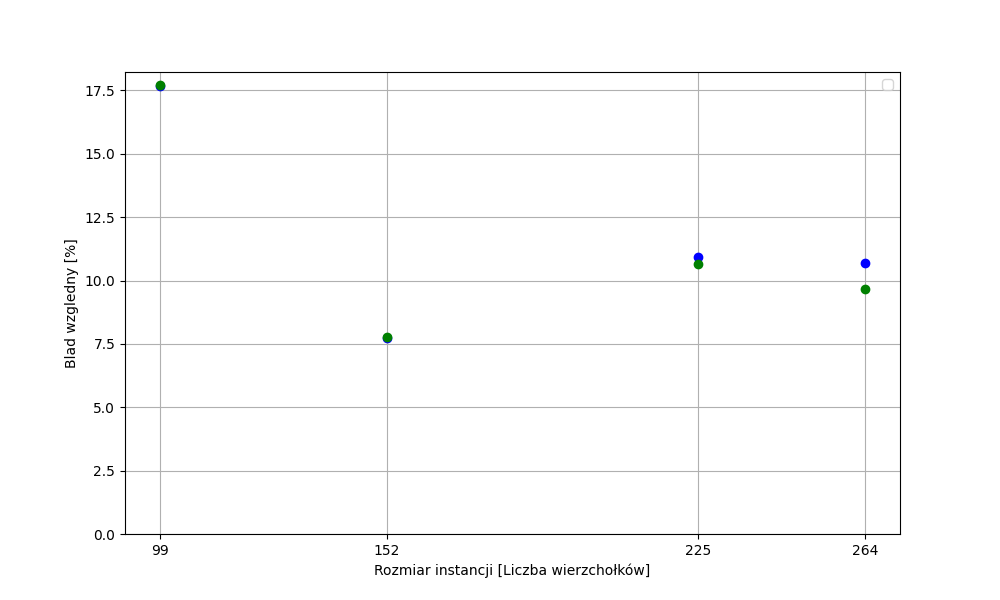
\includegraphics[width=\textwidth]{src/plots/symTsNeighMet.png}
          \caption{Wyniki badań dla macierzy symetrycznych[\%]}
          \label{fig:symNeighg}
        \end{figure}
        \begin{figure}[ht]
          \centering
          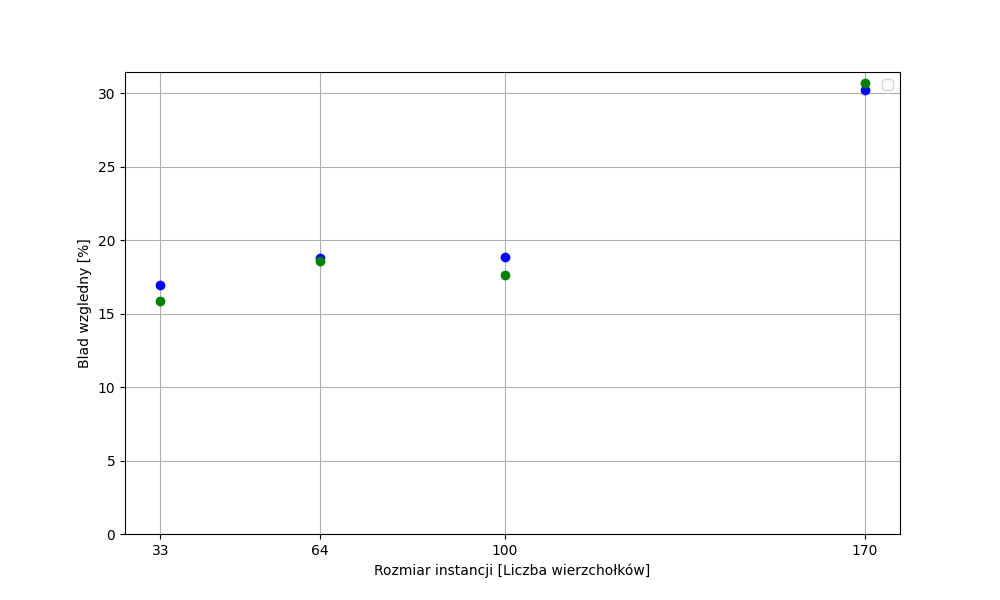
\includegraphics[width=\textwidth]{src/plots/asymTsNeighMet.png}
          \caption{Wyniki badań dla macierzy asymetrycznych[\%]}
          \label{fig:asymNeighg}
        \end{figure}
        \FloatBarrier
        * Niebieskie punkty to wyniki dla Swap a zielone dla Insert
        \textbf{Wnioski: } Wbrew założeniom wyniki są bardzo zbliżone. (\hyperref[tab:error_TsNeighMet]{Tabela 2})
        Różnica nie przekracza 2 punktów procentowych.
      \subsection{Badanie wpływu metody tworzenia pierwszego rozwiązania}
        W moim algorytmie zaimplementowałem dwie różne metody tworzenia pierwszego rozwiązania.
        \begin{enumerate}
          \item Losowa - Pierwsze rozwiązanie jest zupełnie losowe. Najpierw tworzę wektor z liczbami
          od 0 do n - 1. Następnie na tym wektorze używam funkcji shuffle. 
          \item Nearest neighbour - Korzystam z wcześniej zaimplementowanego algorytmu NN. 
        \end{enumerate}
        \textbf{Hipoteza: } Wyniki dla metody losowej będą znacznie gorsze (Większy błąd wzgledny) od NN.
        Ale jest też niewielka szansa na wyniki będące bliżej optymalnego rozwiązania. Jednakże wykonanie
        wielu pomiarów powinno wykluczyć znaczne odstępstwa.\linebreak
        \textbf{Badania: } Podobnie jak w poprzednim przypadku wykonuje badania dla każdej z 8 instancji
        po 4 powtórzenia. Więc znowu wykonuje (4*ASYM + 4*ASM)*4 * 2 = 64\linebreak
        \FloatBarrier
        \begin{table}
\begin{tabular}{|r|r|r|r|r|r|r|r|r|}
\hline
 & \multicolumn{4}{|c|}{Symetryczne} & \multicolumn{4}{|c|}{Asymetryczne} \\ \hline\
Rozmiar[Liczba wierzchołków] & 99 & 152 & 225 & 264 & 33 & 64 & 100 & 170 \\ \hline
NN & 17.67 & 7.75 & 10.93 & 10.71 & 16.95 & 18.76 & 18.86 & 30.20 \\
Random & 436.23 & 1113.25 & 1034.01 & 1921.32 & 82.41 & 256.28 & 318.51 & 730.16 \\ \hline
\end{tabular}
\caption{Błędy w wynikach algorytmu dla macierzy symetrycznych i niesymetrycznych}
\label{tab:error_TsStartVal}
\end{table}

        \FloatBarrier
        \begin{figure}[ht]
          \centering
          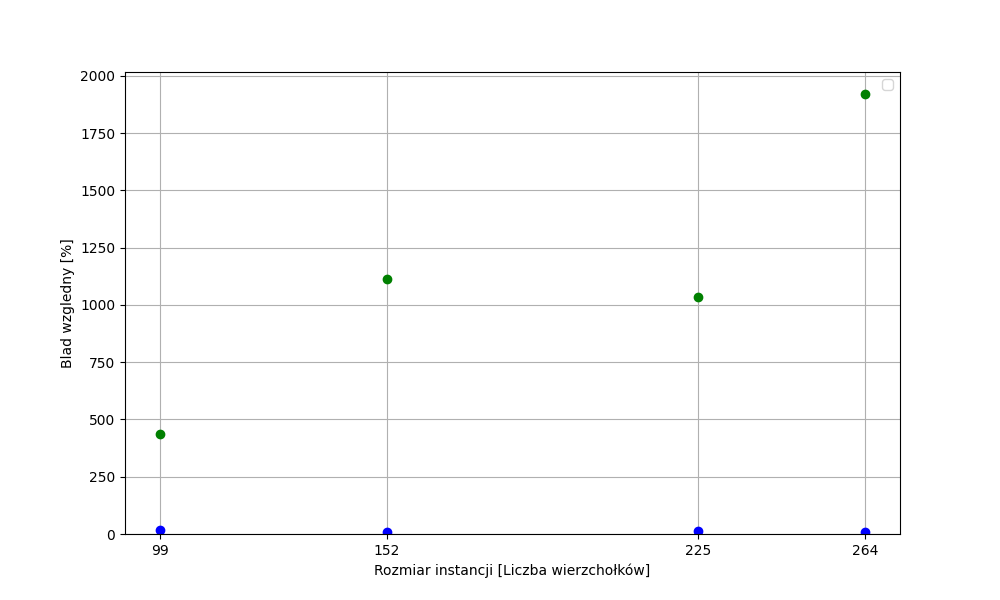
\includegraphics[width=\textwidth]{src/plots/symTsStartVal.png}
          \caption{Wyniki badań dla macierzy symetrycznych}
          \label{fig:symStartVal}
        \end{figure}
        \begin{figure}[ht]
          \centering
          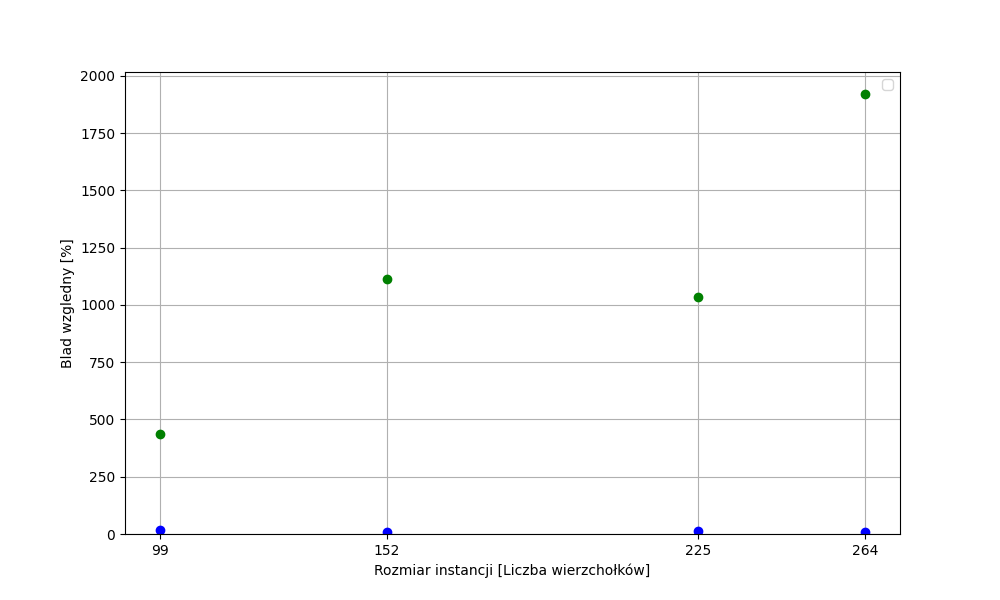
\includegraphics[width=\textwidth]{src/plots/symTsStartVal.png}
          \caption{Wyniki badań dla macierzy asymetrycznych}
          \label{fig:asymStartVal}
        \end{figure}
        \FloatBarrier
        * Niebieskie punkty to wyniki dla NN a zielone dla random.
        \textbf{Wnioski: } Wyniki zgadzają się z moją hipotezą. Było to do przewidzenia
        Jako że random zaczyna w zupełnie losowym punkcie jego rozwiązania będą gorsze.
      \subsection{Badanie wpływu ilości iteracji bez zmian}
        W mojej implementacji przekroczenie pewnej ilości bez zminay wyniku
        służy do dywersyfikacji. Do testów wybrałem wartości 25,50,75,100,125.\linebreak
        \textbf{Hipoteza: } Wraz ze wzrostem ilości iteracji bez zmian jakość
        rozwiązania też będzie rosła.\linebreak
        \textbf{Badania: } Dla każdej instancji testuje wszystkie 5 wartości. 
        Żeby otrzymać dobrą próbkę badanie powtarzam cztero krotnie dla każdej 
        instancji. Dla tego wykonuję (4*ASYM + 4*ASM)*5 * 4 = 160 badań.\linebreak
        \FloatBarrier
        \begin{table}
\begin{tabular}{|r|r|r|r|r|r|r|r|r|}
\hline
 & \multicolumn{4}{|c|}{Symetryczne} & \multicolumn{4}{|c|}{Asymetryczne} \\ \hline\
Rozmiar[Liczba wierzchołków] & 99 & 152 & 225 & 264 & 33 & 64 & 100 & 170 \\ \hline
25 & 17.94 & 7.78 & 10.59 & 9.90 & 15.44 & 18.62 & 17.51 & 30.20 \\
50 & 17.67 & 7.67 & 10.63 & 9.84 & 13.80 & 18.62 & 17.39 & 30.20 \\
75 & 17.86 & 7.64 & 10.66 & 9.79 & 14.50 & 19.24 & 17.33 & 30.20 \\
100 & 17.80 & 7.73 & 10.66 & 10.02 & 15.96 & 18.62 & 18.02 & 30.20 \\
125 & 17.67 & 7.70 & 10.63 & 9.79 & 15.07 & 18.84 & 17.69 & 30.20 \\ \hline
\end{tabular}
\caption{Błędy w wynikach algorytmu dla macierzy symetrycznych i niesymetrycznych}
\label{tab:error_TsCount}
\end{table}

        \FloatBarrier
        \begin{figure}[ht]
          \centering
          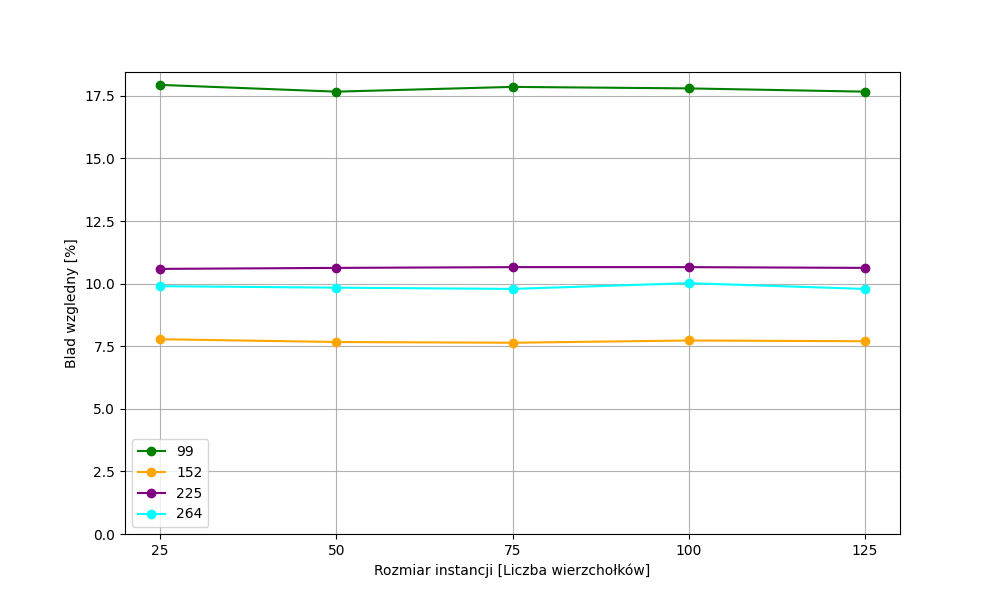
\includegraphics[width=\textwidth]{src/plots/symTsCount.png}
          \caption{Wyniki badań dla macierzy symetrycznych}
          \label{fig:symCount}
        \end{figure}
        \begin{figure}[ht]
          \centering
          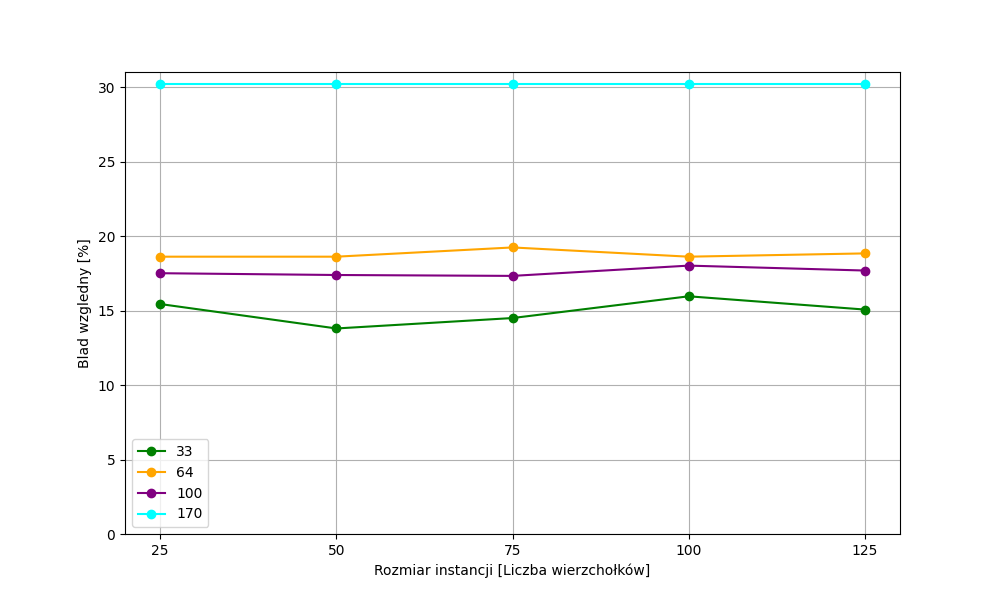
\includegraphics[width=\textwidth]{src/plots/asymTsCount.png}
          \caption{Wyniki badań dla macierzy asymetrycznych}
          \label{fig:asymCount}
        \end{figure}
        \FloatBarrier
        \textbf{Wnioski: } Wyniki są bardzo zbliżone. Różnica dla instancji
        symetrycznych nie jest większa niż 1 punkt procentowy. Dla asymetrycznych
        widać nieco większą różnorodność (ok 2 punkty procentowe). W obu przypadkach
        największy błąd jest dla dużych macierzy
      \subsection{Badanie wpływu długości tablicy tabu} 
        W mojej implementacji elementy pozostają w tablicy tak długo aż 
        ilość elementów w tej tablicy nie przekroczy pewnej liczby. Długość
        tablicy zależna jest od ilości wierzchołków (n * mnożnik).Do testów
        wybrałem wartości 0.5,0.4,0.3,0.2,0.1.\linebreak
        \textbf{Hipoteza: } Jakość rozwiązania powinna rosnąć kiedy długość
        tabeli tabu maleje. Jednakże zbyt mała wartość spowodować cykliczne 
        powracanie do już wygenerowanych rozwiązań.\linebreak
        \textbf{Badania: } Podobnie jak w ostatnim badaniu dla każdej instancji 
        testuje wszystkie 5 wartości. Żeby otrzymać dobrą próbkę badanie 
        powtarzam cztero krotnie dla każdej instancji. Dla tego wykonuję 
        (4*ASYM + 4*ASM)*5 * 4 = 160 badań.\linebreak
        \FloatBarrier
        \begin{table}
\begin{tabular}{|r|r|r|r|r|r|r|r|r|}
\hline
 & \multicolumn{4}{|c|}{Symetryczne} & \multicolumn{4}{|c|}{Asymetryczne} \\ \hline\
Rozmiar[Liczba wierzchołków] & 99 & 152 & 225 & 264 & 33 & 64 & 100 & 170 \\ \hline
0.50 & 18.04 & 7.63 & 10.63 & 9.70 & 14.33 & 18.86 & 17.39 & 30.20 \\
0.40 & 17.80 & 7.70 & 10.66 & 9.46 & 13.43 & 18.56 & 18.22 & 30.20 \\
0.30 & 17.86 & 7.70 & 10.66 & 9.72 & 15.86 & 18.68 & 17.78 & 30.20 \\
0.20 & 17.86 & 7.65 & 10.62 & 9.72 & 14.33 & 18.68 & 17.10 & 30.20 \\
0.10 & 18.02 & 7.63 & 10.70 & 9.57 & 15.82 & 18.56 & 16.90 & 30.20 \\ \hline
\end{tabular}
\caption{Błędy w wynikach algorytmu dla macierzy symetrycznych i niesymetrycznych}
\label{tab:error_TsTabuLen}
\end{table}

        \FloatBarrier
        \begin{figure}[ht]
          \centering
          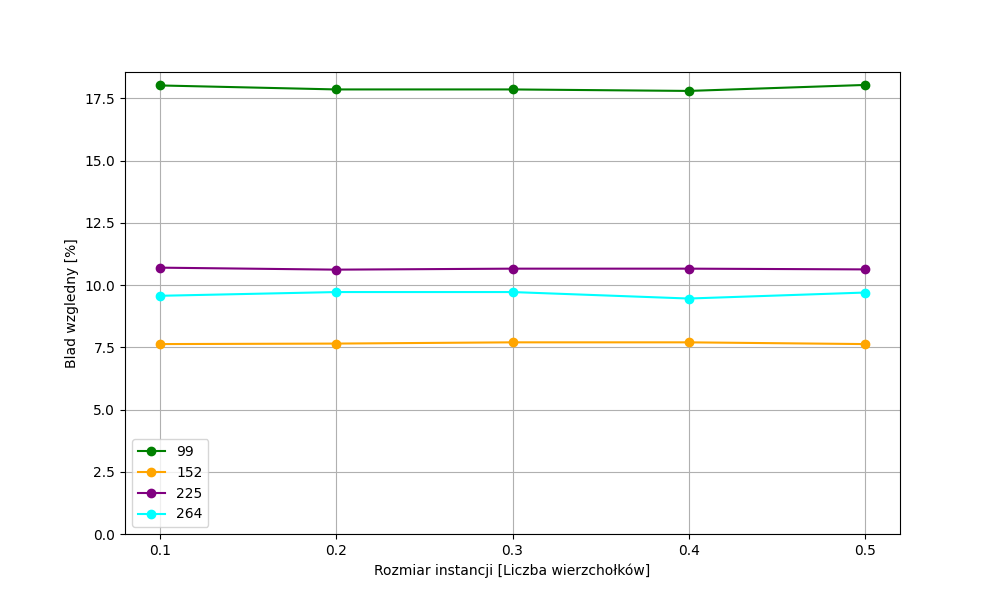
\includegraphics[width=\textwidth]{src/plots/symTsTabuLen.png}
          \caption{Wyniki badań dla macierzy symetrycznych}
          \label{fig:symTabuLen}
        \end{figure}
        \begin{figure}[ht]
          \centering
          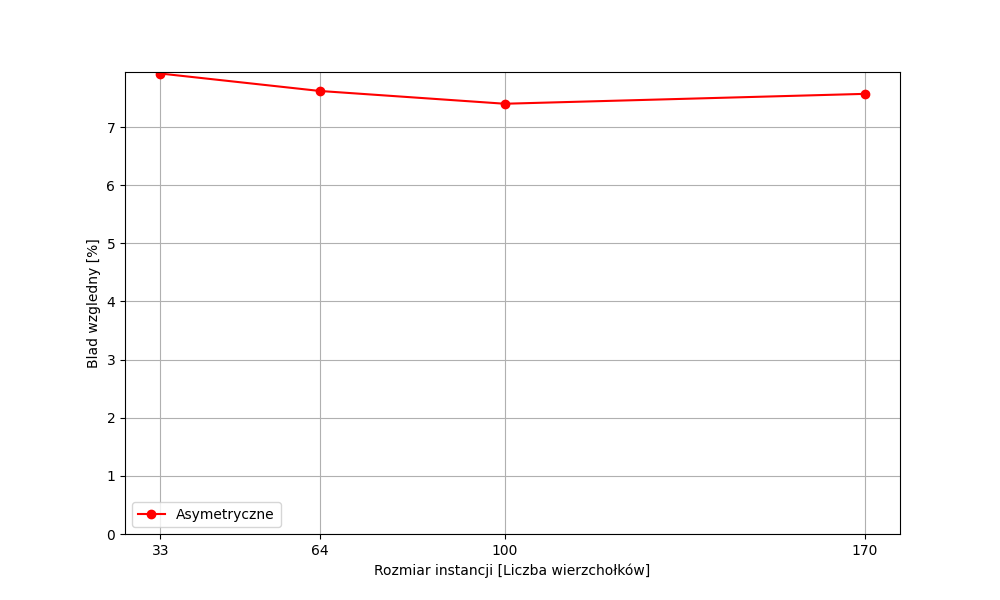
\includegraphics[width=\textwidth]{src/plots/asymTsTabuLen.png}
          \caption{Wyniki badań dla macierzy asymetrycznych}
          \label{fig:asymTabuLen}
        \end{figure}
        \FloatBarrier
        \textbf{Wnioski: } Wyniki są bardzo zbliżone zarówno w tym badaniu jak i 
        w poprzednim. Tak samo jak w poprzednim badaniu wyniki dla macierzy 
        asymetrycznych wykazują znacznie większe zróżnicowanie
      \subsection{Podsumowanie}
        W badaniach 3.4 i 3.5 używałem NN jako metodę tworzenia pierwszego rozwiązania.
        Możliwe że wyniki dla tych instancji były na tyle dobre że algorytm utykał w
        optimum lokalnym.
    \section{Simulated anealing}
      \subsection{Badanie wpływu metody przeszukiwania sąsiedztwa}
        W moim algorytmie zaimplementowałem dwie różne metody przeszukiwania sąsiedztwa.
        \begin{enumerate}
          \item Swap - Wybieram dwa wierzchołki i zamienia je ze sobą. W mojej implementacji
          sprawdzam wszystkie unikalne możliwości więc generuję n*(n-1)/n sąsiadów.
          \item Insert - wybieram wierzchołek i miejsce w tablicy. Wierzchołek kopiuje a następnie 
          usuwam z tablicy. Na koniec kopię wierzchołka wstawiam w wybrane miejsce. W mojej 
          implementacji obie wartości losuję. Wykonuję n*(n-1)/n losowań.
        \end{enumerate}
        \textbf{Hipoteza: } W tabu search metoda przeszukiwania insert powinna być znacznie lepsza
        niż swap.\linebreak
        \textbf{Badania: } Wykonuję badania dla każdej z 8 instancji. Żeby otrzymać dobrą próbkę 
        badanie powtarzam cztero krotnie dla każdej instancji. Więc wykonuje (4*ASYM + 4*ASM)*4 * 2 = 64
        badań. \linebreak
        \FloatBarrier
        \begin{table}
\begin{tabular}{|r|r|r|r|r|r|r|r|r|}
\hline
 & \multicolumn{4}{|c|}{Symetryczne} & \multicolumn{4}{|c|}{Asymetryczne} \\ \hline\
Rozmiar[Liczba wierzchołków] & 99 & 152 & 225 & 264 & 33 & 64 & 100 & 170 \\ \hline
NN & 595.54 & 1295.33 & 1146.48 & 2196.34 & 225.64 & 383.69 & 426.51 & 859.95 \\
Random & 589.22 & 1329.06 & 1135.75 & 2106.88 & 231.53 & 382.49 & 408.62 & 871.63 \\ \hline
\end{tabular}
\caption{Błędy w wynikach algorytmu dla macierzy symetrycznych i niesymetrycznych[\%]}
\label{tab:error_AnNeigMet}
\end{table}

        \FloatBarrier
        \begin{figure}[ht]
          \centering
          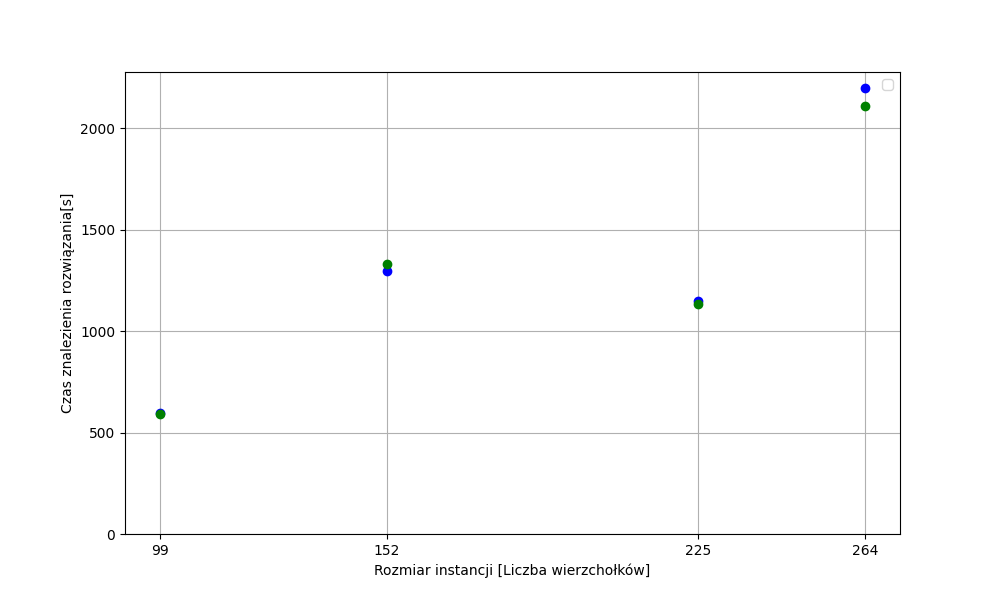
\includegraphics[width=\textwidth]{src/plots/symAnNeigMet.png}
          \caption{Wyniki badań dla macierzy symetrycznych}
          \label{fig:symAnNeig}
        \end{figure}
        \begin{figure}[ht]
          \centering
          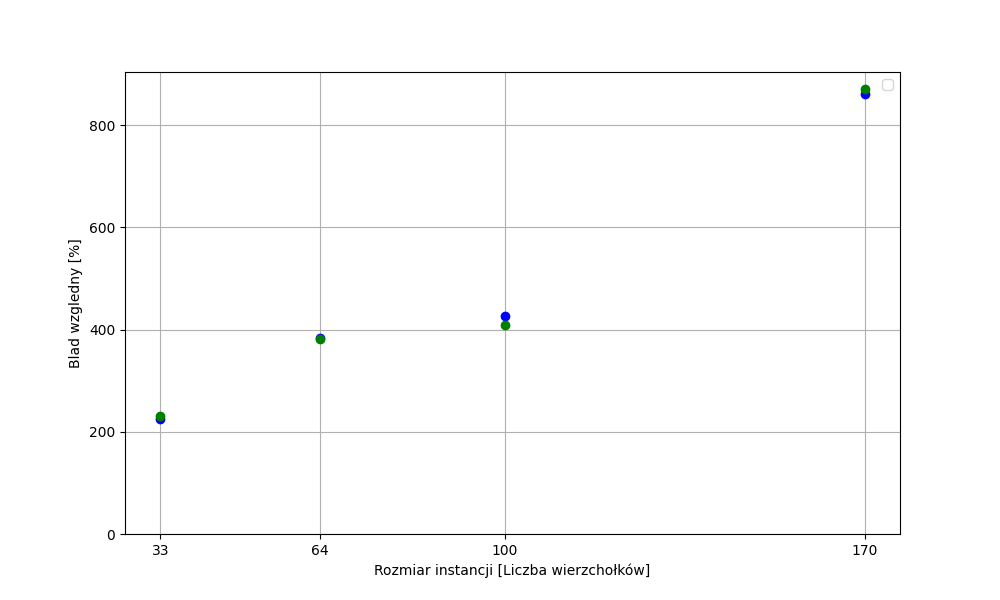
\includegraphics[width=\textwidth]{src/plots/asymAnNeigMet.png}
          \caption{Wyniki badań dla macierzy asymetrycznych}
          \label{fig:asymAnNeig}
        \end{figure}
        \FloatBarrier
        \begin{table}
\begin{tabular}{|r|r|r|r|r|r|r|r|r|}
\hline
 & \multicolumn{4}{|c|}{Symetryczne} & \multicolumn{4}{|c|}{Asymetryczne} \\ \hline\
Rozmiar[Liczba wierzchołków] & 99 & 152 & 225 & 264 & 33 & 64 & 100 & 170 \\ \hline
NN & 0.03 & 0.04 & 0.06 & 0.08 & 0.01 & 0.02 & 0.03 & 0.05 \\
Random & 0.03 & 0.05 & 0.06 & 0.07 & 0.02 & 0.02 & 0.03 & 0.05 \\ \hline
\end{tabular}
\caption{Czas znalezienia wyniku algorytmu dla macierzy symetrycznych i niesymetrycznych[s]}
\label{tab:time_AnNeigMet}
\end{table}

        \FloatBarrier
        \begin{figure}[ht]
          \centering
          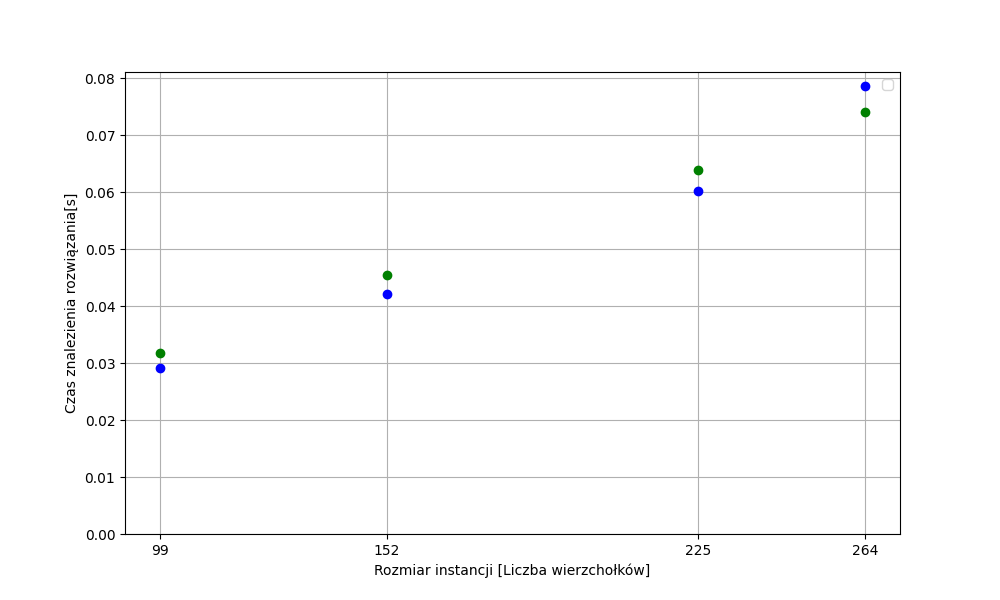
\includegraphics[width=\textwidth]{src/plots/symAnNeigMetTime.png}
          \caption{Wyniki badań czasu  dla macierzy symetrycznych}
          \label{fig:symAnNeigT}
        \end{figure}
        \begin{figure}[ht]
          \centering
          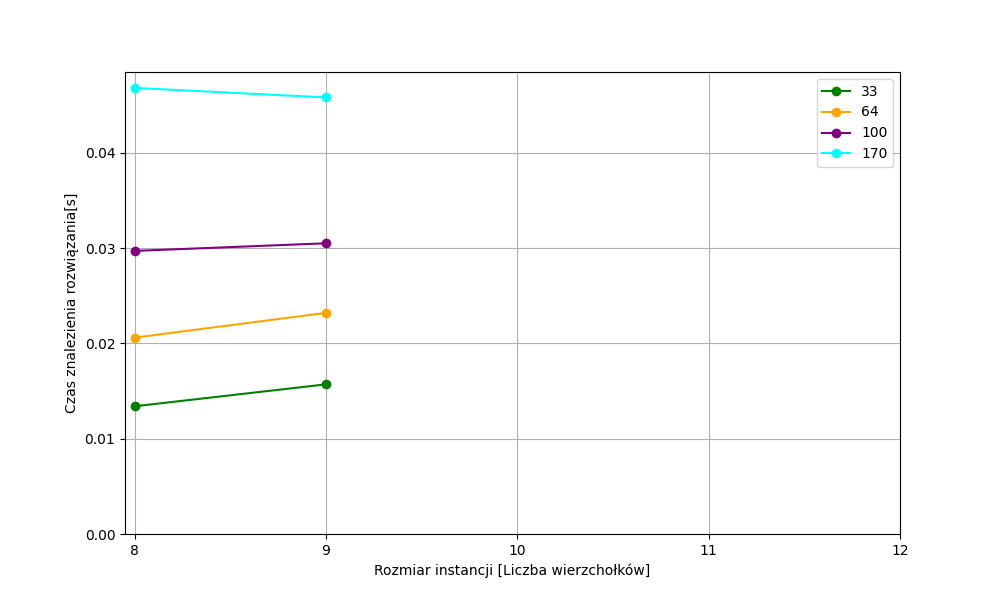
\includegraphics[width=\textwidth]{src/plots/asymAnNeigMetTime.png}
          \caption{Wyniki badań czasu  dla macierzy asymetrycznych}
          \label{fig:asymAnNeigT}
        \end{figure}
        \FloatBarrier
        * Niebieskie punkty to wyniki dla Swap a zielone dla Insert \linebreak
        \textbf{Wnioski: } W tym badaniu błędy dla Random i NN były bardzo zbliżone. Czas znalezienia 
        wyniku dla obu metod jest bardzo zbliżony (różnica ok 0.01 sekundy).
      \subsection{Badanie wpływu metody tworzenia pierwszego rozwiązania}
        W moim algorytmie zaimplementowałem dwie różne metody tworzenia pierwszego rozwiązania.
        \begin{enumerate}
          \item Losowa - Pierwsze rozwiązanie jest zupełnie losowe. Najpierw tworzę wektor z liczbami
          od 0 do n - 1. Następnie na tym wektorze używam funkcji shuffle. 
          \item Nearest neighbour - Korzystam z wcześniej zaimplementowanego algorytmu NN. 
        \end{enumerate}
        \textbf{Hipoteza: } Wyniki dla metody losowej będą znacznie gorsze (Większy błąd wzgledny) od NN.
        Ale jest też niewielka szansa na wyniki będące bliżej optymalnego rozwiązania. Jednakże wykonanie
        wielu pomiarów powinno wykluczyć znaczne odstępstwa.\linebreak
        \textbf{Badania: } Podobnie jak w poprzednim przypadku wykonuje badania dla każdej z 8 instancji
        po 4 powtórzenia. Więc znowu wykonuje (4*ASYM + 4*ASM)*4 * 2 = 64\linebreak
        \FloatBarrier
        \begin{table}
\begin{tabular}{|r|r|r|r|r|r|r|r|r|}
\hline
 & \multicolumn{4}{|c|}{Symetryczne} & \multicolumn{4}{|c|}{Asymetryczne} \\ \hline\
Rozmiar[Liczba wierzchołków] & 99 & 152 & 225 & 264 & 33 & 64 & 100 & 170 \\ \hline
Swap & 579.64 & 1351.90 & 1181.01 & 2143.68 & 223.13 & 389.46 & 430.50 & 853.86 \\
Insert & 601.80 & 1333.36 & 1179.68 & 2157.72 & 233.16 & 353.18 & 428.29 & 867.61 \\ \hline
\end{tabular}
\caption{Błędy w wynikach algorytmu dla macierzy symetrycznych i niesymetrycznych[\%]}
\label{tab:error_AnStartVal}
\end{table}

        \FloatBarrier
        \begin{figure}[ht]
          \centering
          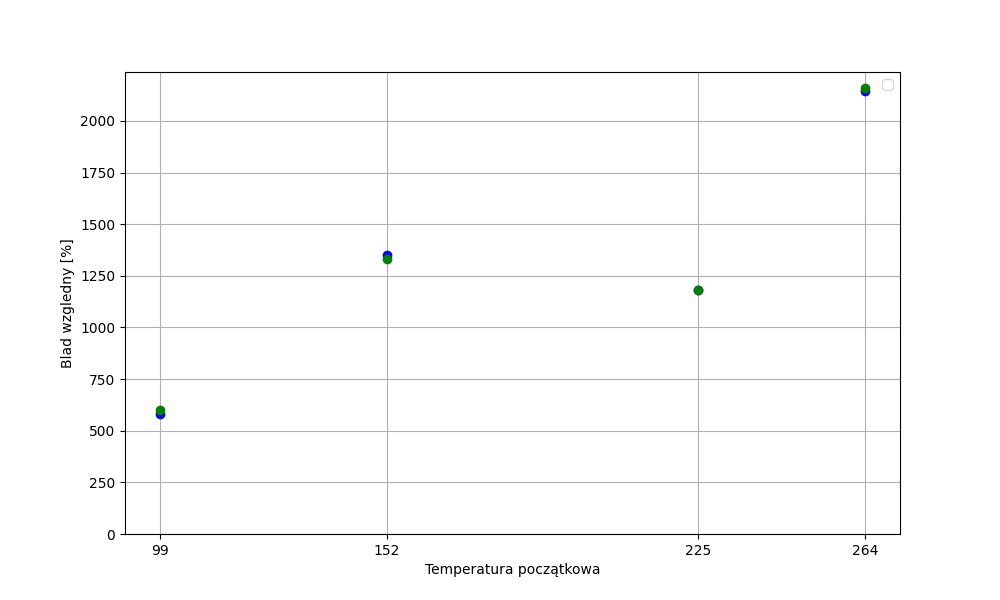
\includegraphics[width=\textwidth]{src/plots/symAnStartVal.png}
          \caption{Wyniki badań dla macierzy symetrycznych}
          \label{fig:symAnStartVal}
        \end{figure}
        \begin{figure}[ht]
          \centering
          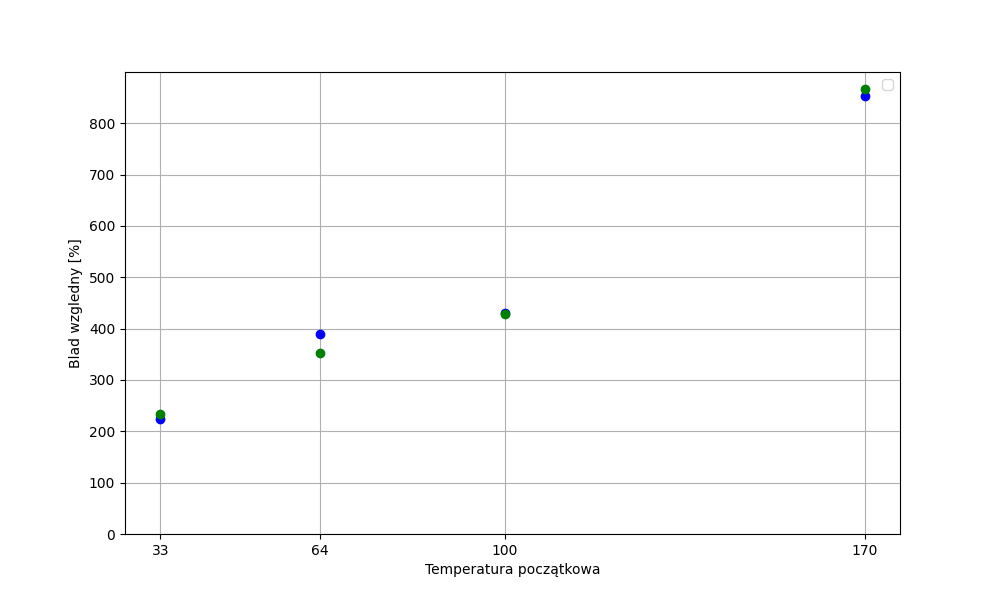
\includegraphics[width=\textwidth]{src/plots/asymAnStartVal.png}
          \caption{Wyniki badań dla macierzy asymetrycznych}
          \label{fig:asymAnStartVal}
        \end{figure}
        \FloatBarrier
        \begin{table}
\begin{tabular}{|r|r|r|r|r|r|r|r|r|}
\hline
 & \multicolumn{4}{|c|}{Symetryczne} & \multicolumn{4}{|c|}{Asymetryczne} \\ \hline\
Rozmiar[Liczba wierzchołków] & 99 & 152 & 225 & 264 & 33 & 64 & 100 & 170 \\ \hline
Swap & 0.03 & 0.04 & 0.06 & 0.08 & 0.01 & 0.02 & 0.03 & 0.05 \\
Insert & 0.03 & 0.04 & 0.06 & 0.08 & 0.01 & 0.02 & 0.03 & 0.05 \\ \hline
\end{tabular}
\caption{Czas znalezienia wyniku algorytmu dla macierzy symetrycznych i niesymetrycznych[s]}
\label{tab:time_AnStartVal}
\end{table}

        \FloatBarrier
        \begin{figure}[ht]
          \centering
          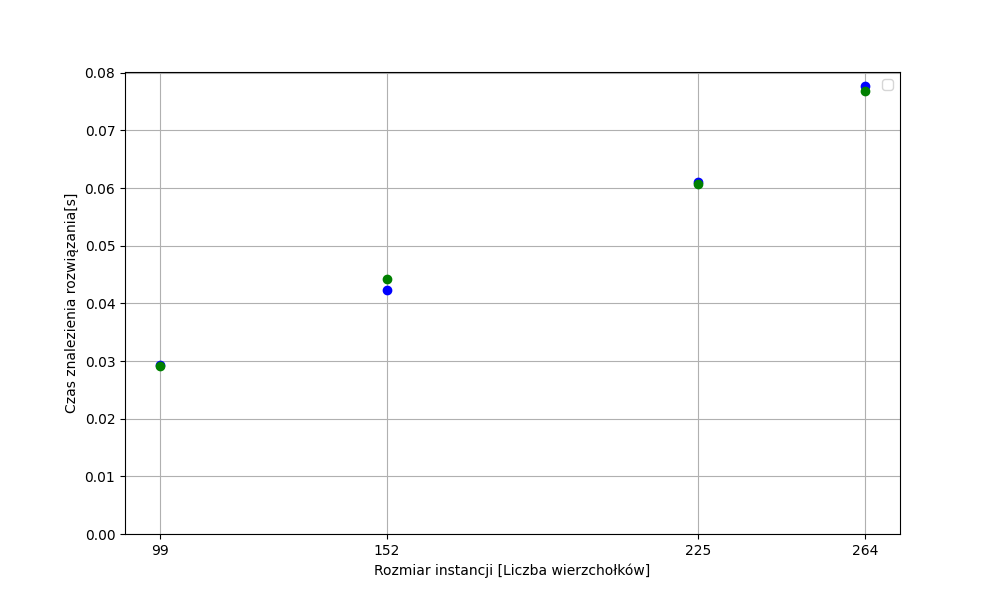
\includegraphics[width=\textwidth]{src/plots/symAnStartValTime.png}
          \caption{Wyniki badań czasu  dla macierzy symetrycznych}
          \label{fig:symStartValT}
        \end{figure}
        \begin{figure}[ht]
          \centering
          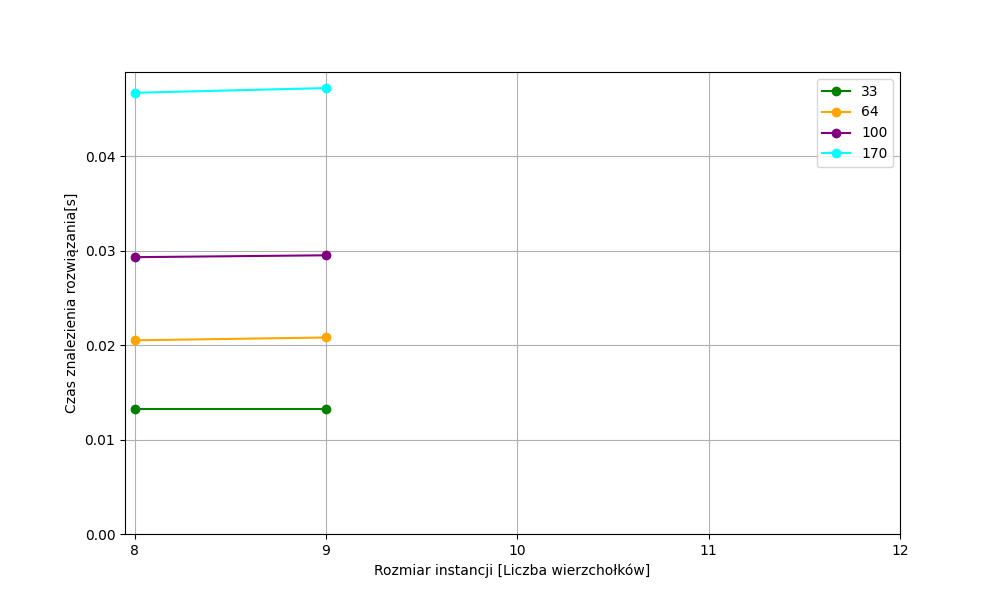
\includegraphics[width=\textwidth]{src/plots/asymAnStartValTime.png}
          \caption{Wyniki badań czasu  dla macierzy asymetrycznych}
          \label{fig:asymStartValT}
        \end{figure}
        \FloatBarrier
        * Niebieskie punkty to wyniki dla Swap a zielone dla Insert\linebreak
        \textbf{Wnioski: } Podobnie jak w badaniu 3.2 wyniki dla obu metod były bardzo
        zbliżone.Czas znalezienia wyniku dla obu metod jest bardzo zbliżony (różnica ok 0.01 sekundy).
      \subsection{Wpływ długości epoki}
        W mojej implementacji długość epoki jest wczytywana z pliku config. 
        Podczas implementacji wartości dla których dostawałem najlepsze
        wyniki były zbliżone do 50. Więc do badań używam wartości 
        20,40,60,80,100.\linebreak
        \textbf{Hipoteza: } Wraz ze wzrostem długości epoki jakość rozwiązania będzie 
        rosła.\linebreak 
        \textbf{Badania: } Dla każdej instancji testuje wszystkie 5 wartości. 
        Żeby otrzymać dobrą próbkę badanie powtarzam cztero krotnie dla każdej 
        instancji. Dla tego wykonuję (4*ASYM + 4*ASM)*5 * 4 = 160 badań.\linebreak 
        \FloatBarrier
        \begin{table}
\begin{tabular}{|r|r|r|r|r|r|r|r|r|}
\hline
 & \multicolumn{4}{|c|}{Symetryczne} & \multicolumn{4}{|c|}{Asymetryczne} \\ \hline\
Rozmiar[Liczba wierzchołków] & 99 & 152 & 225 & 264 & 33 & 64 & 100 & 170 \\ \hline
20 & 597.40 & 1360.05 & 1155.71 & 2156.53 & 237.89 & 352.66 & 438.31 & 840.99 \\
40 & 592.80 & 1293.06 & 1189.70 & 2210.11 & 197.05 & 373.48 & 450.66 & 861.12 \\
60 & 574.75 & 1369.14 & 1148.52 & 2120.59 & 220.45 & 377.23 & 418.36 & 843.57 \\
80 & 590.40 & 1405.35 & 1156.42 & 2190.91 & 219.54 & 377.60 & 417.86 & 840.92 \\
100 & 593.13 & 1384.52 & 1142.86 & 2207.36 & 217.07 & 381.70 & 411.56 & 853.87 \\ \hline
\end{tabular}
\caption{Błędy w wynikach algorytmu dla macierzy symetrycznych i niesymetrycznych[\%]}
\label{tab:error_AnEpoch}
\end{table}

        \FloatBarrier
        \begin{figure}[ht]
          \centering
          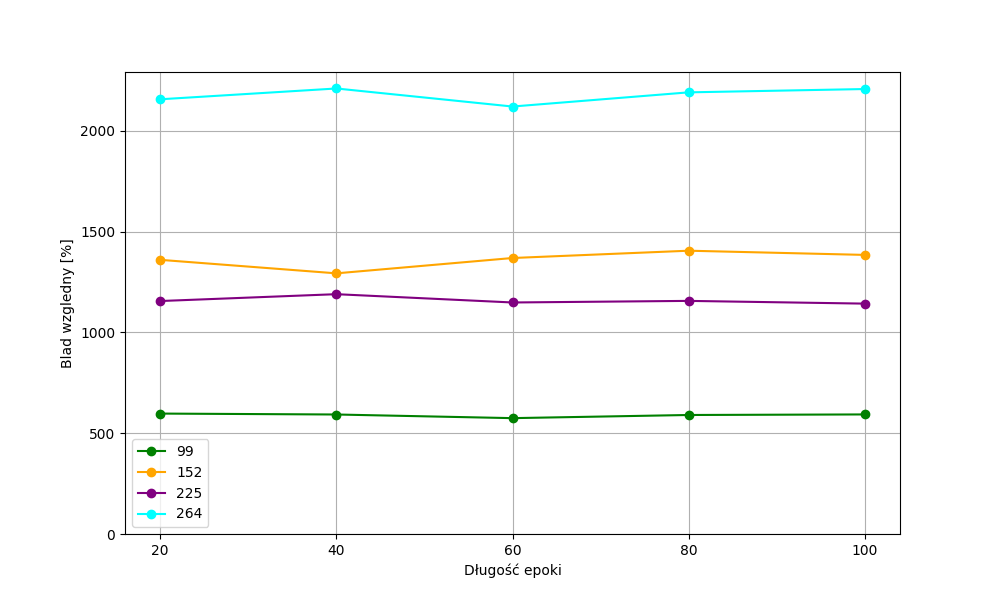
\includegraphics[width=\textwidth]{src/plots/symAnEpoch.png}
          \caption{Wyniki badań dla macierzy symetrycznych}
          \label{fig:symEpoch}
        \end{figure}
        \begin{figure}[ht]
          \centering
          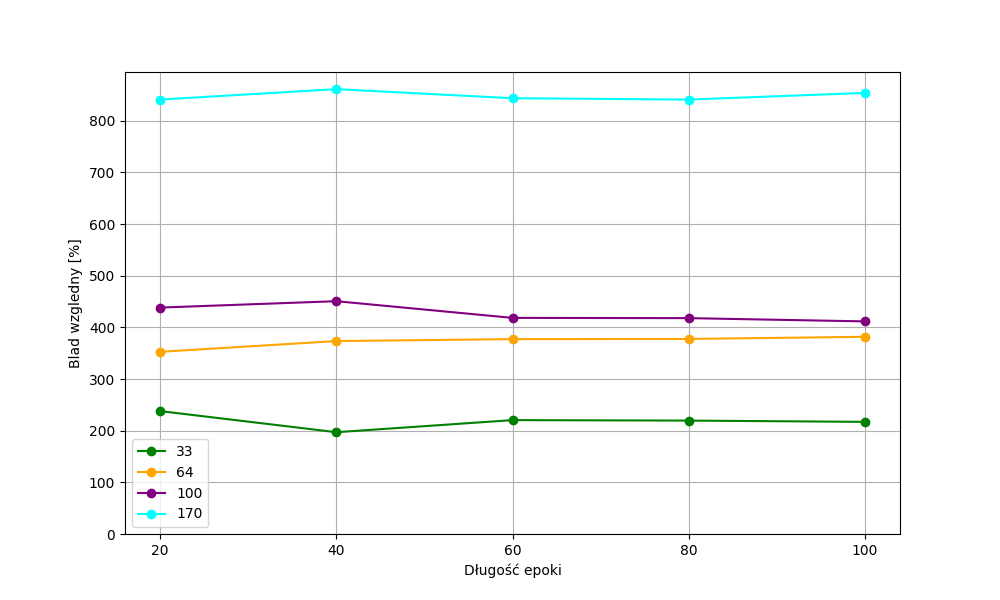
\includegraphics[width=\textwidth]{src/plots/asymAnEpoch.png}
          \caption{Wyniki badań dla macierzy asymetrycznych}
          \label{fig:asymEpoch}
        \end{figure}
        \FloatBarrier
        \begin{table}
\begin{tabular}{|r|r|r|r|r|r|r|r|r|}
\hline
 & \multicolumn{4}{|c|}{Symetryczne} & \multicolumn{4}{|c|}{Asymetryczne} \\ \hline\
Rozmiar[Liczba wierzchołków] & 99 & 152 & 225 & 264 & 33 & 64 & 100 & 170 \\ \hline
20 & 0.01 & 0.02 & 0.03 & 0.04 & 0.01 & 0.01 & 0.02 & 0.02 \\
40 & 0.03 & 0.04 & 0.06 & 0.07 & 0.02 & 0.02 & 0.03 & 0.05 \\
60 & 0.05 & 0.07 & 0.09 & 0.12 & 0.02 & 0.03 & 0.05 & 0.08 \\
80 & 0.06 & 0.09 & 0.13 & 0.15 & 0.03 & 0.05 & 0.06 & 0.10 \\
100 & 0.08 & 0.11 & 0.16 & 0.20 & 0.04 & 0.06 & 0.08 & 0.12 \\ \hline
\end{tabular}
\caption{Czas znalezienia wyniku algorytmu dla macierzy symetrycznych i niesymetrycznych[s]}
\label{tab:time_AnEpoch}
\end{table}

        \FloatBarrier
        \begin{figure}[ht]
          \centering
          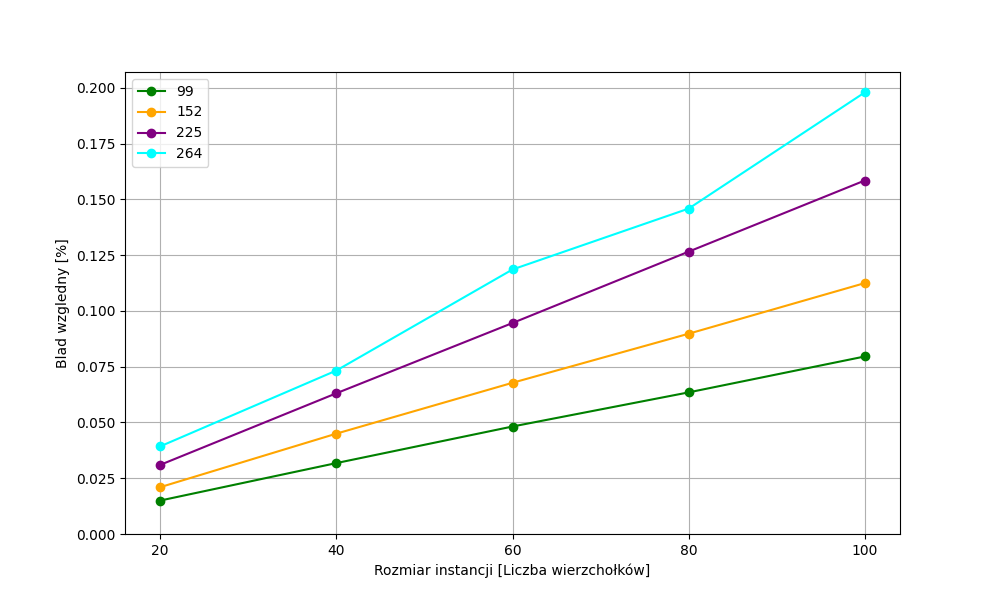
\includegraphics[width=\textwidth]{src/plots/symAnEpochTime.png}
          \caption{Wyniki badań czasu  dla macierzy symetrycznych}
          \label{fig:symEpochT}
        \end{figure}
        \begin{figure}[ht]
          \centering
          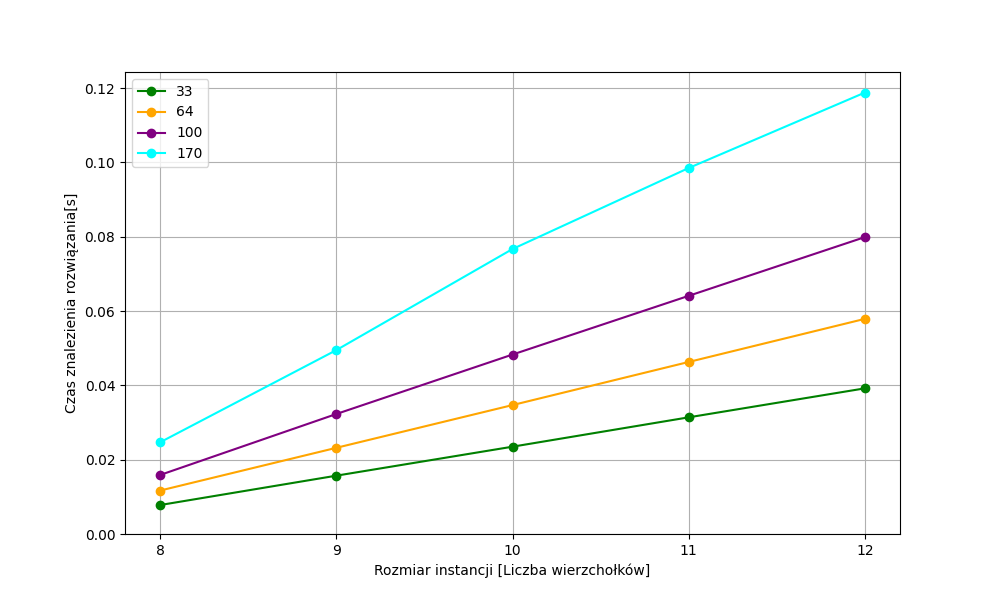
\includegraphics[width=\textwidth]{src/plots/asymAnEpochTime.png}
          \caption{Wyniki badań czasu dla macierzy asymetrycznych}
          \label{fig:asymEpochT}
        \end{figure}
        \FloatBarrier
        \textbf{Wnioski: } Z badania wynikia że czas rośnie liniowo w raz ze wzrostem 
        długości epok. Dla wszyskich długości epok różnica w błędzie była niewielka.
        Jednakże otrzymany błąd był bardzo duży ok 800\%
      \subsection{Wielkość alfa}
        W mojej implementacji wartość alfa jest wczytywana z pliku config. Alfa powinna
        być w zakresie 0 do 1. Więc do testów wybrałem wartości 0.19,0.39,0.59,0.79,0.99. \linebreak
        \textbf{Hipoteza: } Wraz ze wzrostem wartości alfy wyniki powinny się poprawiać.
        Alfa = 0.99 powinna dawać najlepsze wyniki.\linebreak
        \textbf{Badania: } Dla każdej instancji testuje wszystkie 5 wartości. 
        Żeby otrzymać dobrą próbkę badanie powtarzam cztero krotnie dla każdej 
        instancji. Dla tego wykonuję (4*ASYM + 4*ASM)*5 * 4 = 160 badań.\linebreak
        \FloatBarrier
        \begin{table}
\begin{tabular}{|r|r|r|r|r|r|r|r|r|}
\hline
 & \multicolumn{4}{|c|}{Symetryczne} & \multicolumn{4}{|c|}{Asymetryczne} \\ \hline\
Rozmiar[Liczba wierzchołków] & 99 & 152 & 225 & 264 & 33 & 64 & 100 & 170 \\ \hline
0.19 & 566.49 & 1324.13 & 1176.88 & 2220.35 & 232.64 & 359.73 & 433.55 & 822.99 \\
0.39 & 598.93 & 1346.84 & 1157.42 & 2214.13 & 235.19 & 376.70 & 426.96 & 872.64 \\
0.59 & 619.05 & 1289.91 & 1166.79 & 2155.45 & 237.17 & 362.15 & 432.80 & 851.40 \\
0.79 & 605.90 & 1296.39 & 1167.63 & 2154.71 & 222.38 & 378.22 & 424.60 & 864.62 \\
0.99 & 589.66 & 1332.67 & 1161.08 & 2171.91 & 238.16 & 388.88 & 424.59 & 866.60 \\ \hline
\end{tabular}
\caption{Błędy w wynikach algorytmu dla macierzy symetrycznych i niesymetrycznych[\%]}
\label{tab:error_AnAlpha}
\end{table}

        \FloatBarrier
        \begin{figure}[ht]
          \centering
          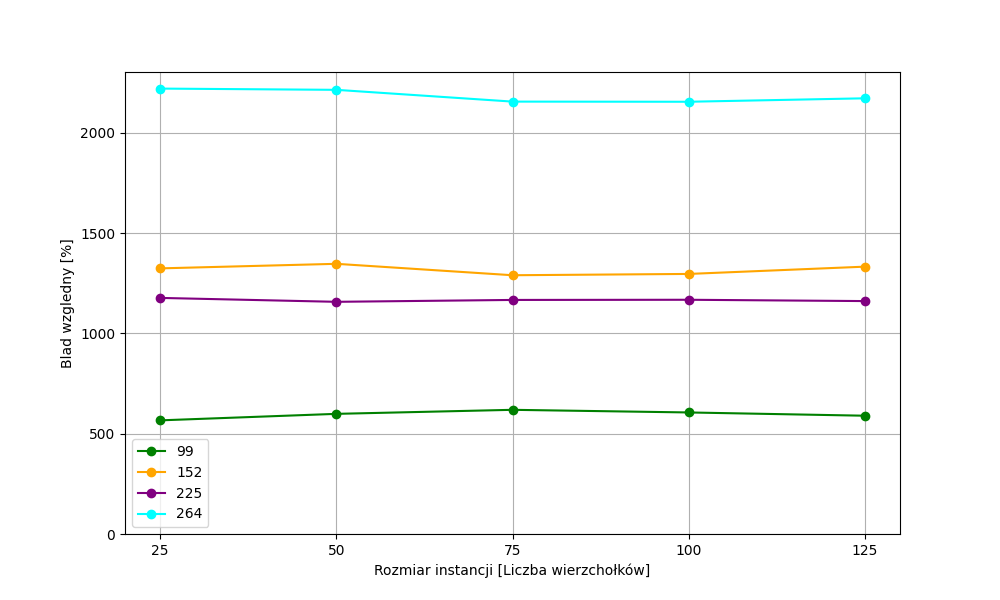
\includegraphics[width=\textwidth]{src/plots/symAnAlpha.png}
          \caption{Wyniki badań dla macierzy symetrycznych}
          \label{fig:symAlpha}
        \end{figure}
        \begin{figure}[ht]
          \centering
          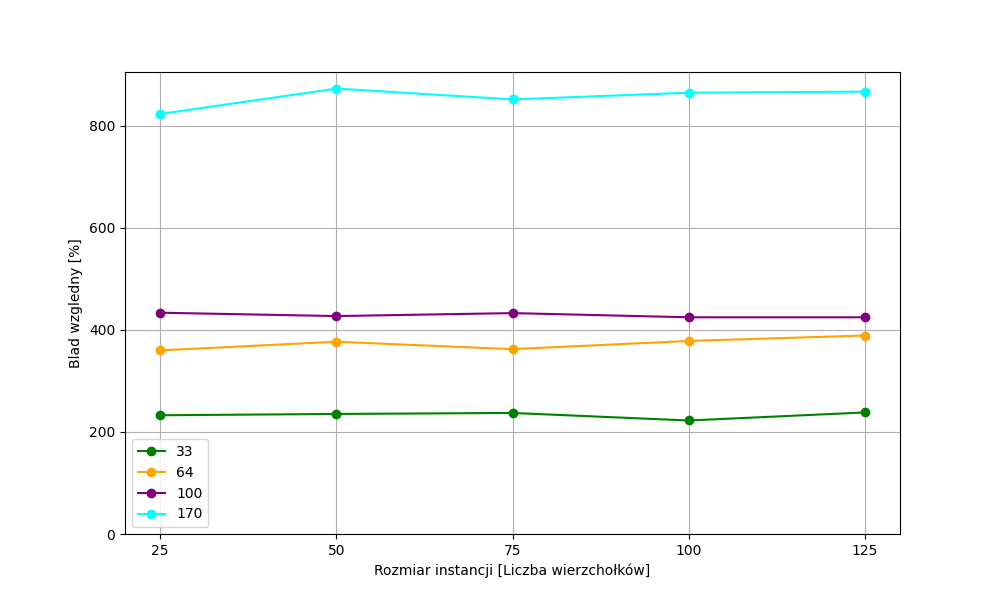
\includegraphics[width=\textwidth]{src/plots/asymAnAlpha.png}
          \caption{Wyniki badań dla macierzy asymetrycznych}
          \label{fig:asymAlphan}
        \end{figure}
        \FloatBarrier
        \begin{table}
\begin{tabular}{|r|r|r|r|r|r|r|r|r|}
\hline
 & \multicolumn{4}{|c|}{Symetryczne} & \multicolumn{4}{|c|}{Asymetryczne} \\ \hline\
Rozmiar[Liczba wierzchołków] & 99 & 152 & 225 & 264 & 33 & 64 & 100 & 170 \\ \hline
0.19 & 0.00 & 0.00 & 0.00 & 0.00 & 0.00 & 0.00 & 0.00 & 0.00 \\
0.39 & 0.00 & 0.00 & 0.00 & 0.00 & 0.00 & 0.00 & 0.00 & 0.00 \\
0.59 & 0.00 & 0.00 & 0.00 & 0.00 & 0.00 & 0.00 & 0.00 & 0.00 \\
0.79 & 0.00 & 0.00 & 0.00 & 0.01 & 0.00 & 0.00 & 0.00 & 0.00 \\
0.99 & 0.01 & 0.01 & 0.01 & 0.02 & 0.00 & 0.01 & 0.01 & 0.01 \\ \hline
\end{tabular}
\caption{Czas znalezienia wyniku algorytmu dla macierzy symetrycznych i niesymetrycznych[s]}
\label{tab:time_AnAlpha}
\end{table}

        \FloatBarrier
        \begin{figure}[ht]
          \centering
          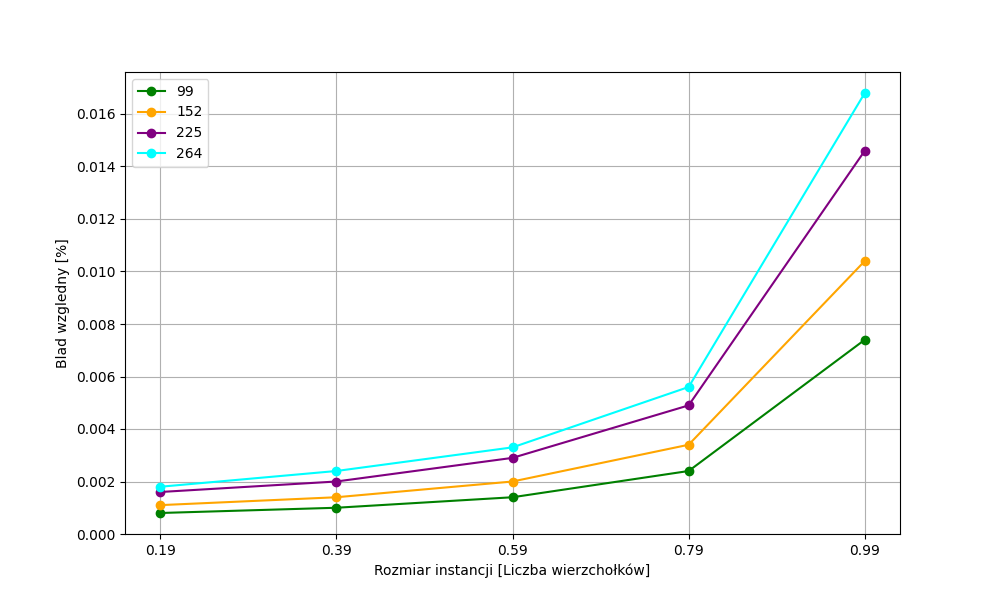
\includegraphics[width=\textwidth]{src/plots/symAnAlphaTime.png}
          \caption{Wyniki badań dla macierzy symetrycznych}
          \label{fig:symAlphaT}
        \end{figure}
        \begin{figure}[ht]
          \centering
          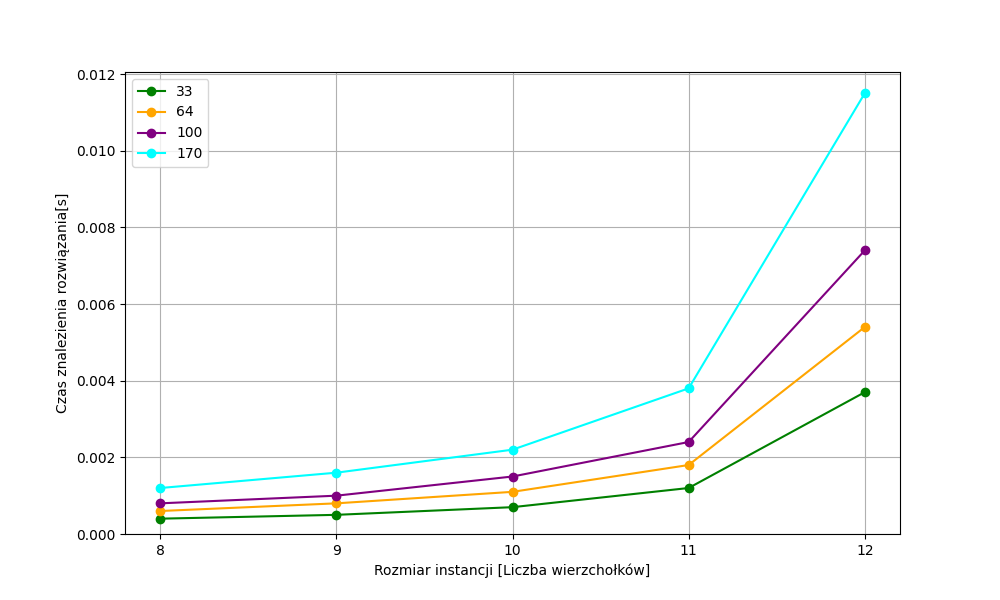
\includegraphics[width=\textwidth]{src/plots/asymAnAlphaTime.png}
          \caption{Wyniki badań dla macierzy asymetrycznych}
          \label{fig:asymAlphaT}
        \end{figure}
        \FloatBarrier 
        \textbf{Wnioski: } Różnica błędów dla wartości alfy była nieznacznia ok 10 punktów procentowych.
        Czas znalezienia rozwiązań znacznie poprawiał się dla małych wartości alfa. Czas potrzebny na
        znalezienie wyniku rośnie wykładniczo kiedy alfa zbliża się do 1.
      \subsection{Temperatura startowa}
        W mojej implementacji temperatura startowa jest wczytywana z pliku config.
        Podczas implementacji temperatura startowa zbliżona do 5000 dawała najlepsze 
        wyniki. Więc do badań wybrałem wartości 1000,2000,3000,4000,5000.\linebreak
        \textbf{Hipoteza: } Temperatura startowa powinna być stosunkowo wysoka
        więc wraz ze wzrostem wyniki powinny się poprawiać.\linebreak
        \textbf{Badania: } Dla każdej instancji testuje wszystkie 5 wartości. 
        Żeby otrzymać dobrą próbkę badanie powtarzam cztero krotnie dla każdej 
        instancji. Dla tego wykonuję (4*ASYM + 4*ASM)*5 * 4 = 160 badań.\linebreak
        \FloatBarrier
        \begin{table}
\begin{tabular}{|r|r|r|r|r|r|r|r|r|}
\hline
 & \multicolumn{4}{|c|}{Symetryczne} & \multicolumn{4}{|c|}{Asymetryczne} \\ \hline\
Rozmiar[Liczba wierzchołków] & 99 & 152 & 225 & 264 & 33 & 64 & 100 & 170 \\ \hline
1000 & 605.51 & 1312.89 & 1159.97 & 2199.02 & 240.14 & 382.42 & 429.30 & 857.04 \\
2000 & 618.21 & 1354.90 & 1176.62 & 2170.17 & 200.86 & 378.47 & 417.61 & 842.63 \\
3000 & 610.92 & 1351.52 & 1139.70 & 2210.24 & 229.72 & 377.42 & 421.46 & 845.69 \\
4000 & 591.21 & 1324.39 & 1164.62 & 2185.20 & 229.16 & 375.01 & 442.47 & 862.23 \\
5000 & 579.54 & 1332.35 & 1165.11 & 2118.00 & 230.79 & 367.01 & 438.10 & 833.51 \\ \hline
\end{tabular}
\caption{Błędy w wynikach algorytmu dla macierzy symetrycznych i niesymetrycznych[\%]}
\label{tab:error_AnStart}
\end{table}

        \FloatBarrier
        \begin{figure}[ht]
          \centering
          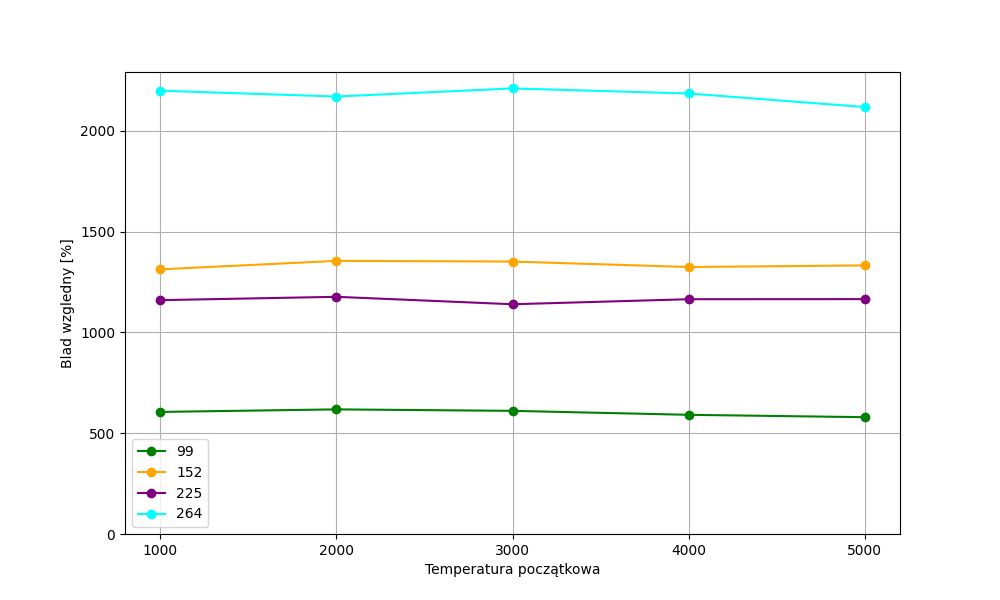
\includegraphics[width=\textwidth]{src/plots/symAnStart.png}
          \caption{Wyniki badań dla macierzy symetrycznych}
          \label{fig:symStart}
        \end{figure}
        \begin{figure}[ht]
          \centering
          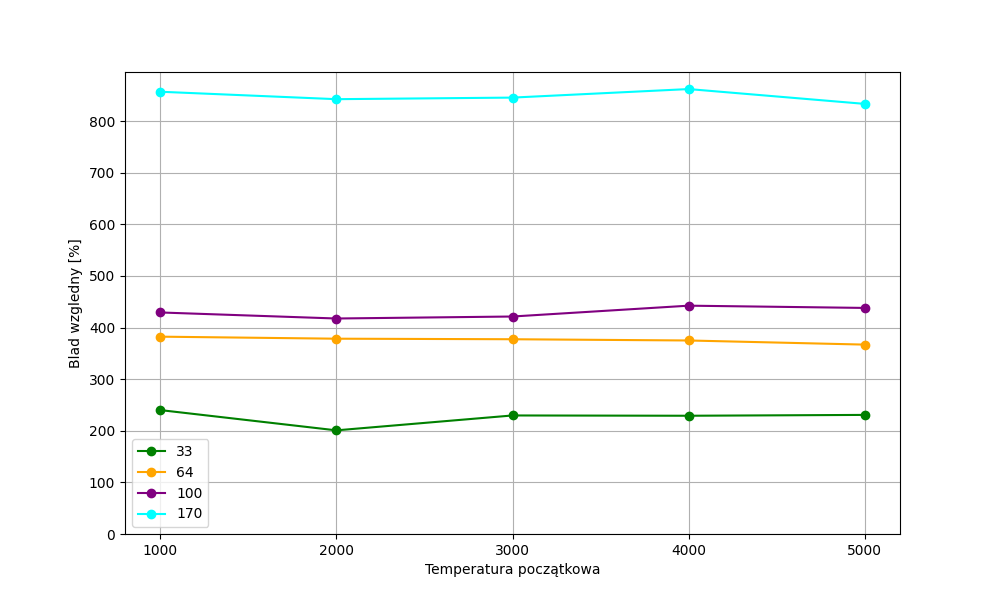
\includegraphics[width=\textwidth]{src/plots/asymAnStart.png}
          \caption{Wyniki badań dla macierzy asymetrycznych}
          \label{fig:asymStart}
        \end{figure}
        \FloatBarrier
        \begin{table}
\centering
\begin{tabular}{|r|r|r|r|r|r|r|r|r|r|r|}
\hline
 & \multicolumn{4}{|c|}{Symetryczne} & \multicolumn{4}{|c|}{Asymetryczne} \\ \hline\
Rozmiar & 99 & 152 & 225 & 264 & 33 & 64 & 100 & 170 \\ \hline
8 & 0.007 & 0.009 & 0.013 & 0.015 & 0.003 & 0.005 & 0.006 & 0.010 \\
9 & 0.007 & 0.009 & 0.013 & 0.015 & 0.003 & 0.005 & 0.007 & 0.011 \\
10 & 0.007 & 0.010 & 0.014 & 0.016 & 0.003 & 0.005 & 0.007 & 0.011 \\
11 & 0.007 & 0.010 & 0.014 & 0.016 & 0.004 & 0.005 & 0.007 & 0.011 \\
12 & 0.007 & 0.010 & 0.014 & 0.016 & 0.004 & 0.005 & 0.007 & 0.011 \\ \hline
\end{tabular}
\caption{Czas znalezienia wyniku algorytmu dla macierzy symetrycznych i niesymetrycznych[s]}
\label{tab:time_AnStart}
\end{table}

        \FloatBarrier
        \begin{figure}[ht]
          \centering
          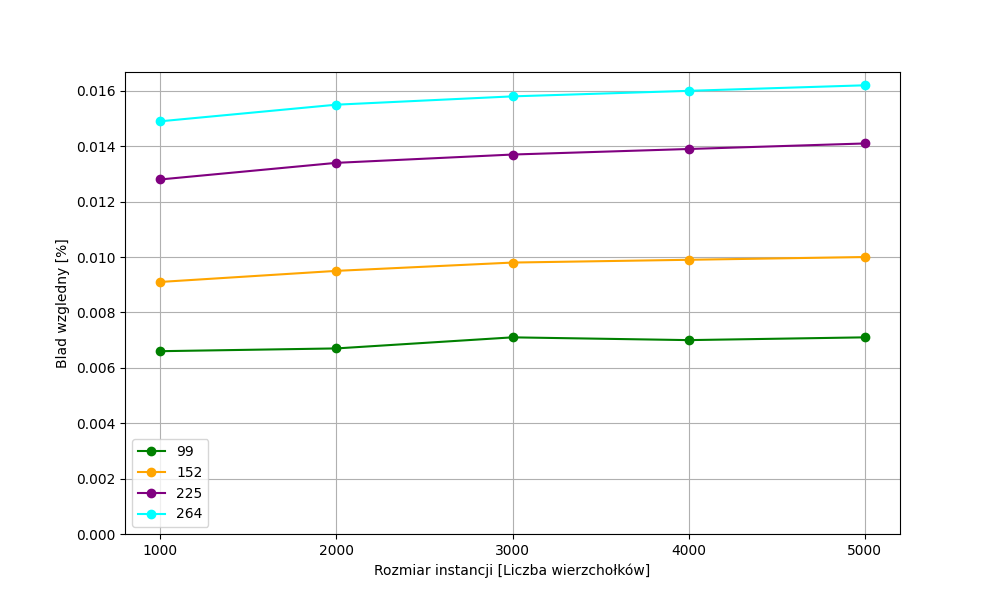
\includegraphics[width=\textwidth]{src/plots/symAnStartTime.png}
          \caption{Wyniki badań dla macierzy symetrycznych}
          \label{fig:symStartT}
        \end{figure}
        \begin{figure}[ht]
          \centering
          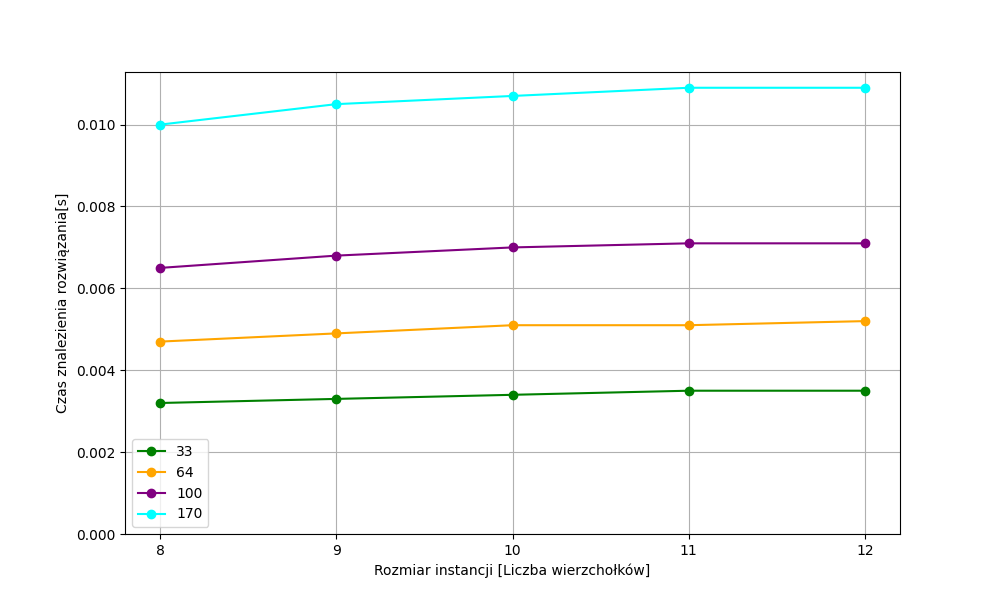
\includegraphics[width=\textwidth]{src/plots/asymAnStartTime.png}
          \caption{Wyniki badań dla macierzy asymetrycznych}
          \label{fig:asymStartT}
        \end{figure}
        \FloatBarrier
        \textbf{Wnioski: } Podobnie jak ostatnio różnica między błędami dla kolejnych
        wartości początkowych. Tym razem czas znalezienia rozwiązania też nie różnił się
        znacząco ok 0.01s.        
      \subsection{Podsumowanie}
        Różnice które powstają przy stosowani różnych parametrów są znacznie lepiej widoczne 
        kiedy badamy czas otrzymania najlepszego wyniku. Niestety błąd wzgledny dla tego algorytmu
        możliwe że w implementacji pojawiły się błędy.
    \section{Algorytm mrówkowy}
      \subsection{Opis Algorytmu}
        Algorytm mrówkwy jest algorytmem metahurystycznym który modeluje zachowanie mrówek.
        Mrówki w wyruszają z mrowiska w poszukiwaniu jedzenia w losowych kierunkach. Po 
        znalezieniu jedzenia mrówki wracają do mrowiska i pozostawiają za sobą feromony.
        Ilość zostawionych feromonów zależy od ilości znalezionego jedzenia. Następnie
        mrówki ponownie wyruszają z mrowiska ścieżki wybierają z pewnym prawdopodobieństwem
        które zależy od ilości feromonów. Jako że feromony parują to ścieżki nie uczęszczane
        zanikają a te prowadzące do dobrych rozwiązań są wzmacniane.\linebreak
        W mojej implementacji ścieżki wybierane są z pewnym prawdopodobieństwem 
        wyliczonym ze wzoru:  \[
            p_{ij}^k(t) = \frac{a_{ij}(t)}{\sum{l\in N_i}a_{il}(t)}
        \]
        Gdzie k to k-ta mrówka ;a i , j to ścieżka z i-tego wierzchołka do j-tego.
        Natomiast wartości początkowe feromonów szacowane są ze wzoru $\tau_0 = \frac{k}{C^{nn}}$
        W tym wzorze $C^{nn}$ to wynik algorytmu NN dla tej instancji.
      \subsection{Badanie wpływu typu rozkładu feromonów}
        W mojej implementacji mam dwa typy rozkładu feromonów
        \begin{enumerate}
          \item CAS - Algorytm cykliczny aktualizuje wartości feromonów po 
          wybraniu całej ścieżki. Aktualizacja przebiega według wzoru 
          $\delta \tau_{ij}^k(t,t+n) = n/L^k$ gdzie $L^k$ to długość otrzymanej trasy.
          \item QAS - Algorytm ilościowy aktualizuje wartości feromonów po 
          wybraniu krawędzi Aktualizacja przebiega według wzoru 
          $\delta \tau_{ij}^k(t,t+n) = n/d_{ij}$ gdzie $d_{ij}$ to koszt przejścia
          z i do j.\linebreak
        \end{enumerate}
        \textbf{Hipoteza: } Algorytm QAS powinien dawać nieznacznie lepsze wyniki.\linebreak
        \textbf{Badania: } Dla obu metod wykonuje badania dla każdej z 8 
        instancji, powtarzam je cztero krotnie by otrzymać dobrą próbkę.
        Więc wykonuje (4*ASYM + 4*ASM)*2 * 4 = 64 badań.\linebreak
        \FloatBarrier
        \begin{table}
\centering
\begin{tabular}{|r|r|r|r|r|r|r|r|r|r|r|}
\hline
 & \multicolumn{6}{|c|}{Symetryczne} & \multicolumn{4}{|c|}{Asymetryczne} \\ \hline\
Rozmiar & 99 & 152 & 225 & 264 & 318 & 439 & 33 & 64 & 100 & 170 \\ \hline
QAS & 18.660 & 7.980 & 10.930 & 10.900 & 17.060 & 18.670 & 17.420 & 19.740 & 19.560 & 36.190 \\
CAS & 18.660 & 7.980 & 10.930 & 10.900 & 17.060 & 18.670 & 17.420 & 19.740 & 19.560 & 36.190 \\ \hline
\end{tabular}
\caption{Błędy w wynikach algorytmu dla macierzy symetrycznych i niesymetrycznych[\%]}
\label{tab:error_AoFeroMet}
\end{table}

        \FloatBarrier
        \begin{figure}[ht]
          \centering
          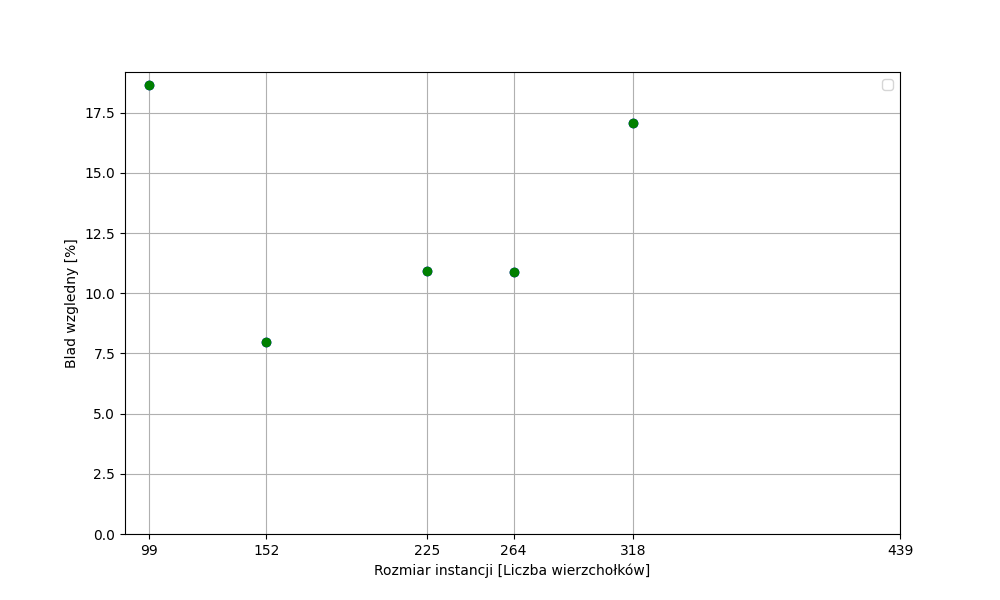
\includegraphics[width=\textwidth]{src/plots/symAoFeroMet.png}
          \caption{Wyniki badań dla macierzy symetrycznych}
          \label{fig:symFero}
        \end{figure}
        \begin{figure}[ht]
          \centering
          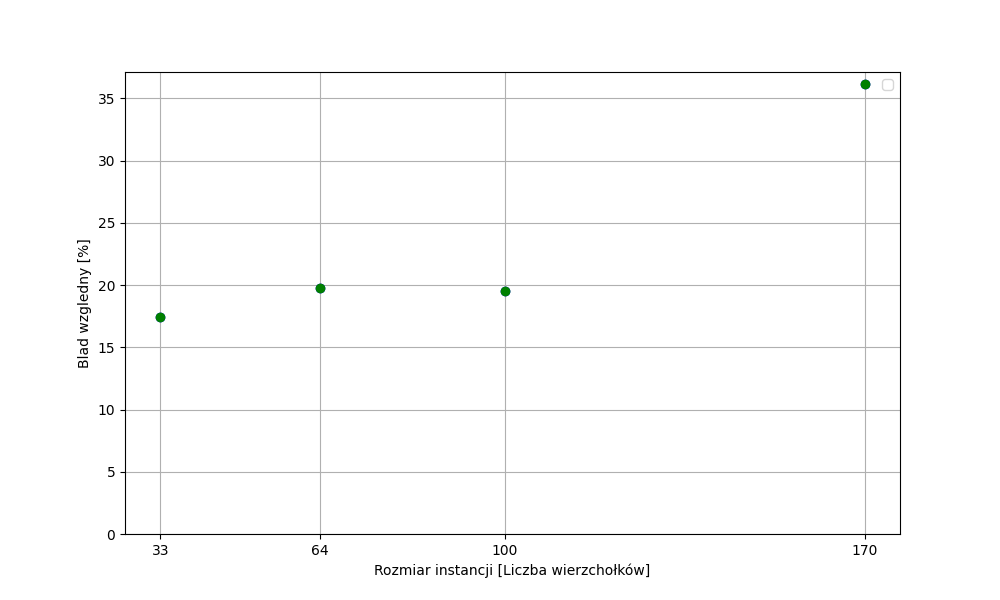
\includegraphics[width=\textwidth]{src/plots/asymAoFeroMet.png}
          \caption{Wyniki badań dla macierzy asymetrycznych}
          \label{fig:asymFero}
        \end{figure}
        \FloatBarrier
        \begin{table}
\centering
\begin{tabular}{|r|r|r|r|r|r|r|r|r|r|r|}
\hline
 & \multicolumn{6}{|c|}{Symetryczne} & \multicolumn{4}{|c|}{Asymetryczne} \\ \hline\
Rozmiar & 99 & 152 & 225 & 264 & 318 & 439 & 33 & 64 & 100 & 170 \\ \hline
QAS & 0.009 & 0.049 & 0.220 & 0.413 & 0.850 & 3.038 & 0.000 & 0.002 & 0.010 & 0.074 \\
CAS & 0.009 & 0.048 & 0.218 & 0.408 & 0.846 & 3.026 & 0.000 & 0.002 & 0.010 & 0.074 \\ \hline
\end{tabular}
\caption{Czas znalezienia wyniku algorytmu dla macierzy symetrycznych i niesymetrycznych[s]}
\label{tab:time_AoFeroMet}
\end{table}

        \FloatBarrier
        \begin{figure}[ht]
          \centering
          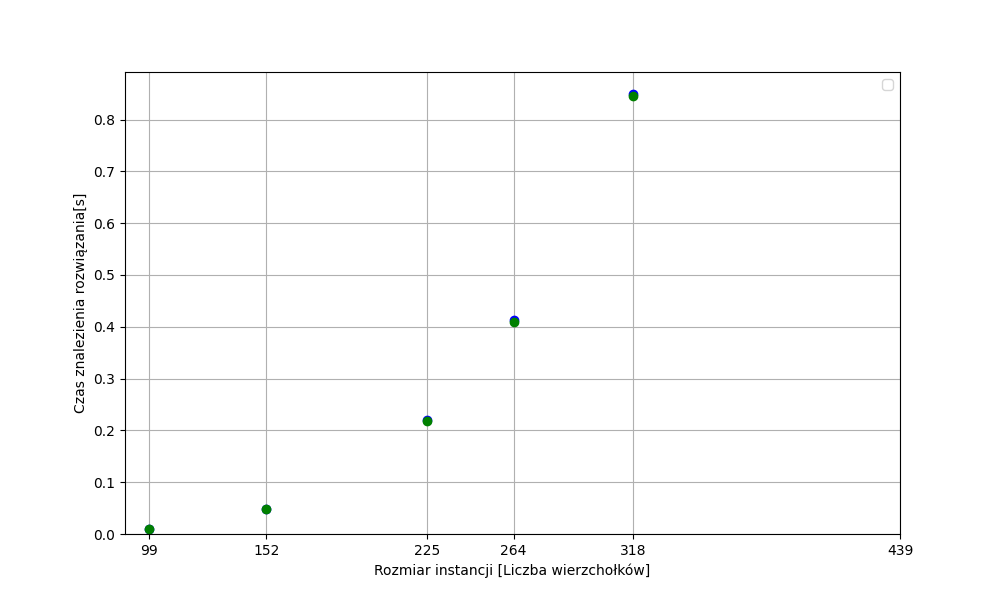
\includegraphics[width=\textwidth]{src/plots/symAoFeroMetTime.png}
          \caption{Wyniki badań dla macierzy symetrycznych}
          \label{fig:symFeroT}
        \end{figure}
        \begin{figure}[ht]
          \centering
          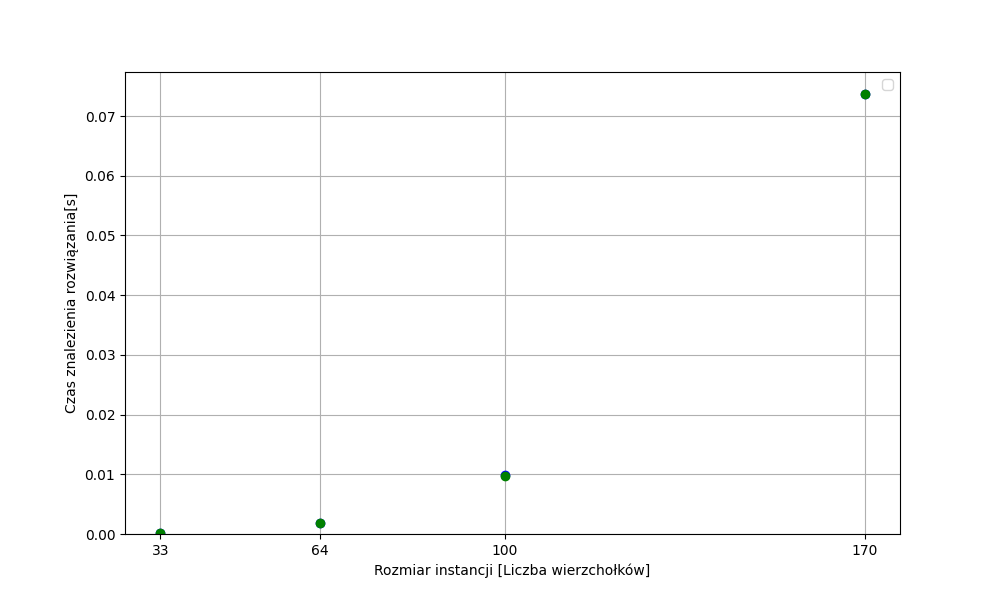
\includegraphics[width=\textwidth]{src/plots/asymAoFeroMetTime.png}
          \caption{Wyniki badań dla macierzy asymetrycznych}
          \label{fig:asymFeroT}
        \end{figure}
        \FloatBarrier
        * Niebieskie punkty to wyniki dla Swap a zielone dla Insert\linebreak
        \textbf{Wnioski: } Dla obu zaimplementowanych algorytmów (CAS i QAS) błąd względny
        jest bardzo podobny (w większości przypadków taki sam). Czas potrzebny na znalezienie
        rozwiązania rośnie wykładniczo.
      \subsection{Badanie wpływu wartości rho}
        Wartość $\rho$ to współczynnik parowania feromonów. Po tym jak wszystkie
        mrówki wybrały swoją ścieżkę wartości feromonów są przemnażane przez $\rho$.
        Dlatego też wartości $\rho$ powinny być w zakresie 0 do 1. Dlatego wybrałem
        wartości 0.8,0.6,0.4,0.2\linebreak
        \textbf{Hipoteza: } Wysokie wartości $\rho$ powinny zachęcać mrówki do wybierania
        różnych nie koniecznie optymalnych ścieżek. Natomiast niskie wartości powinny 
        sprawiać że mrówki będą bardziej zachłannne\linebreak
        \textbf{Badania: } Dla każdej instancji testuje wszystkie 5 wartości. 
        Żeby otrzymać dobrą próbkę badanie powtarzam cztero krotnie dla każdej 
        instancji. Dla tego wykonuję (4*ASYM + 4*ASM)*5 * 4 = 160 badań.\linebreak
        \FloatBarrier
        \begin{table}
\centering
\begin{tabular}{|r|r|r|r|r|r|r|r|r|r|r|}
\hline
 & \multicolumn{6}{|c|}{Symetryczne} & \multicolumn{4}{|c|}{Asymetryczne} \\ \hline\
Rozmiar & 99 & 152 & 225 & 264 & 318 & 439 & 33 & 64 & 100 & 170 \\ \hline
0.100 & 18.660 & 7.980 & 10.930 & 10.900 & 17.060 & 18.670 & 17.420 & 19.740 & 19.560 & 36.190 \\
0.200 & 18.660 & 7.980 & 10.930 & 10.900 & 17.060 & 18.670 & 17.420 & 19.740 & 19.560 & 36.190 \\
0.300 & 18.660 & 7.980 & 10.930 & 10.900 & 17.060 & 18.670 & 17.420 & 19.740 & 19.560 & 36.190 \\
0.400 & 18.660 & 7.980 & 10.930 & 10.900 & 17.060 & 18.670 & 17.420 & 19.740 & 19.560 & 36.190 \\
0.500 & 18.660 & 7.980 & 10.930 & 10.900 & 17.060 & 18.670 & 17.420 & 19.740 & 19.560 & 36.190 \\ \hline
\end{tabular}
\caption{Błędy w wynikach algorytmu dla macierzy symetrycznych i niesymetrycznych[\%]}
\label{tab:error_AoRho}
\end{table}

        \FloatBarrier
        \begin{figure}[ht]
          \centering
          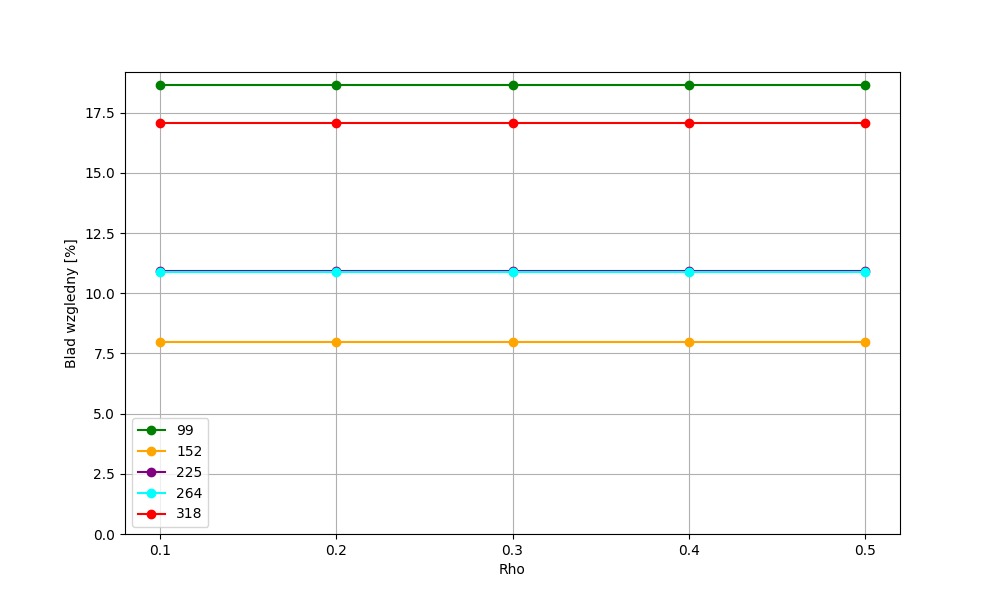
\includegraphics[width=\textwidth]{src/plots/symAoRho.png}
          \caption{Wyniki badań dla macierzy symetrycznych}
          \label{fig:symRho}
        \end{figure}
        \begin{figure}[ht]
          \centering
          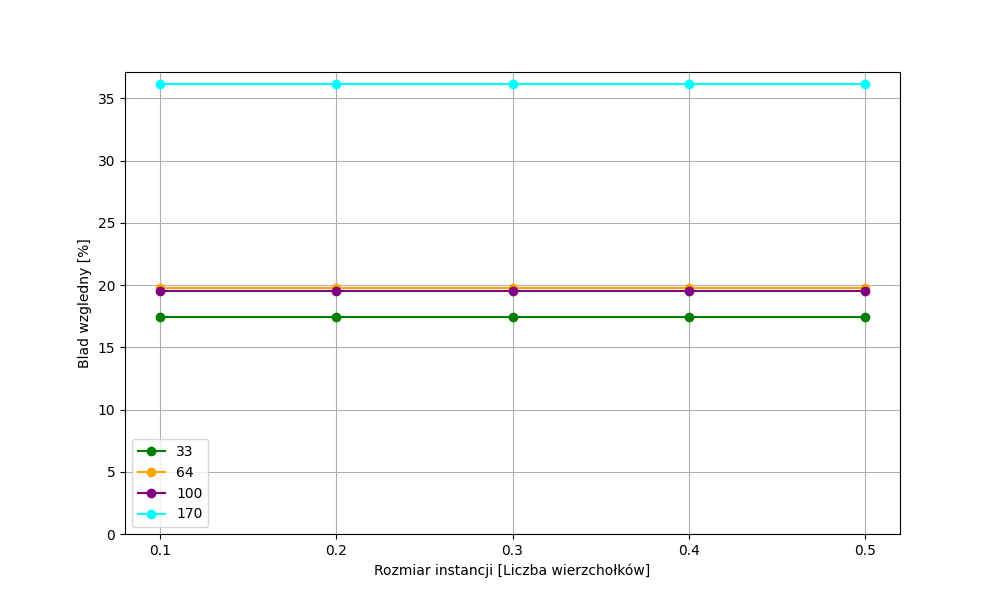
\includegraphics[width=\textwidth]{src/plots/asymAoRho.png}
          \caption{Wyniki badań dla macierzy asymetrycznych}
          \label{fig:asymRho}
        \end{figure}
        \FloatBarrier
        \begin{table}
\centering
\begin{tabular}{|r|r|r|r|r|r|r|r|r|r|r|}
\hline
 & \multicolumn{6}{|c|}{Symetryczne} & \multicolumn{4}{|c|}{Asymetryczne} \\ \hline\
Rozmiar & 99 & 152 & 225 & 264 & 318 & 439 & 33 & 64 & 100 & 170 \\ \hline
0.100 & 0.009 & 0.049 & 0.221 & 0.409 & 0.851 & 3.019 & 0.000 & 0.002 & 0.010 & 0.074 \\
0.200 & 0.009 & 0.048 & 0.222 & 0.429 & 0.852 & 3.031 & 0.000 & 0.002 & 0.010 & 0.074 \\
0.300 & 0.009 & 0.048 & 0.219 & 0.408 & 0.845 & 3.026 & 0.000 & 0.002 & 0.010 & 0.074 \\
0.400 & 0.009 & 0.048 & 0.220 & 0.410 & 0.851 & 3.026 & 0.000 & 0.002 & 0.010 & 0.074 \\
0.500 & 0.009 & 0.048 & 0.219 & 0.412 & 0.855 & 3.012 & 0.000 & 0.002 & 0.010 & 0.074 \\ \hline
\end{tabular}
\caption{Czas znalezienia wyniku algorytmu dla macierzy symetrycznych i niesymetrycznych[s]}
\label{tab:time_AoRho}
\end{table}

        \FloatBarrier
        \begin{figure}[ht]
          \centering
          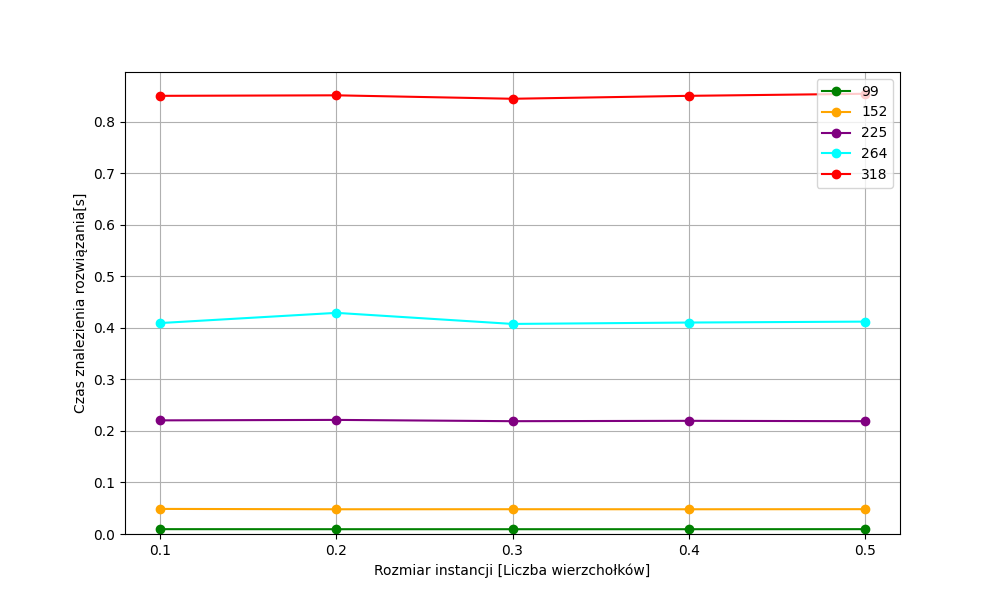
\includegraphics[width=\textwidth]{src/plots/symAoRhoTime.png}
          \caption{Wyniki badań dla macierzy symetrycznych}
          \label{fig:symRhoT}
        \end{figure}
        \begin{figure}[ht]
          \centering
          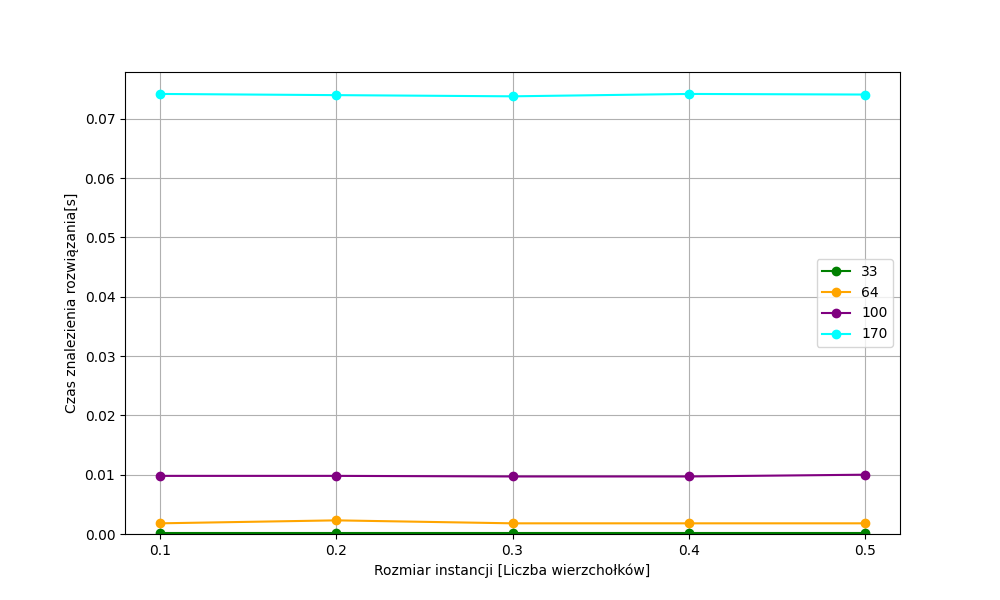
\includegraphics[width=\textwidth]{src/plots/asymAoRhoTime.png}
          \caption{Wyniki badań dla macierzy asymetrycznych}
          \label{fig:asymRhoT}
        \end{figure}
        \FloatBarrier
        \textbf{Wnioski: } W otrzymanych wynikach nie ma większych różnic dla różnych wartości rho.
        Może to być spowodowane miejscem w którym feromony parują (Po wyliczeniu ścieżek dla wszyskich mrówek).
      \subsection{Badanie wpływu stosunku alfy do bety}
        W mojej implementacji używam tablic decyzyjnych gdzie \[ A_i = [a_{ij} (t)]_{Ni}\]
        Wartości $A_i$ wyliczam na początku nowego pokolenia. Natomiast elementy $a_{ij}$
        wyliczam ze wzoru:
        \[
            a_{ij}t = \frac{[\tau_{ij}(t)]^\alpha*[\tau_{ij}(t)]^\beta}{\sum{l\in N_i}[\tau_{ij}(t)]^\alpha*[\tau_{ij}(t)]^\beta}
        \]
        Do testów wybrałem 5 wartości $\frac{\alpha}{\beta}$ $\frac{1}{3},\frac{2}{3},1,\frac{3}{2},3$\linebreak
        \textbf{Hipoteza: } Zwiększając element $\alpha$ zwiększa się szansa na wybranie ścieżki z dużą 
        ilością feromonów. Natomiast Zwiększając $\beta$ zwiększa się szansa na wybranie ścieżki z niewielką
        ilością feromonów. Kiedy $\alpha = \beta$ wynik będzie najgorszy. Ale dla małego $\alpha$ i dużego
        $\beta$ powinien być najlepszy. \linebreak
        \textbf{Badania: } Dla każdej instancji testuje wszystkie 5 wartości. 
        Żeby otrzymać dobrą próbkę badanie powtarzam cztero krotnie dla każdej 
        instancji. Dla tego wykonuję (4*ASYM + 4*ASM)*5 * 4 = 160 badań.\linebreak
        \FloatBarrier
        \begin{table}
\centering
\begin{tabular}{|r|r|r|r|r|r|r|r|r|r|r|}
\hline
 & \multicolumn{6}{|c|}{Symetryczne} & \multicolumn{4}{|c|}{Asymetryczne} \\ \hline\
Rozmiar & 99 & 152 & 225 & 264 & 318 & 439 & 33 & 64 & 100 & 170 \\ \hline
1/3 & 18.660 & 7.980 & 10.930 & 10.900 & 17.060 & 18.670 & 17.420 & 19.740 & 19.560 & 36.190 \\
2/3 & 18.660 & 7.980 & 10.930 & 10.900 & 17.060 & 18.670 & 17.420 & 19.740 & 19.560 & 36.190 \\
1 & 18.660 & 7.980 & 10.930 & 10.900 & 17.060 & 18.670 & 16.410 & 19.740 & 19.560 & 36.190 \\
3/2 & 18.660 & 7.980 & 10.930 & 10.900 & 17.060 & 18.670 & 17.420 & 19.740 & 19.560 & 36.190 \\
3 & 18.660 & 7.980 & 10.930 & 10.900 & 17.060 & 18.670 & 17.420 & 19.740 & 19.560 & 36.190 \\ \hline
\end{tabular}
\caption{Błędy w wynikach algorytmu dla macierzy symetrycznych i niesymetrycznych[\%]}
\label{tab:error_AoAB}
\end{table}

        \FloatBarrier
        \begin{figure}[ht]
          \centering
          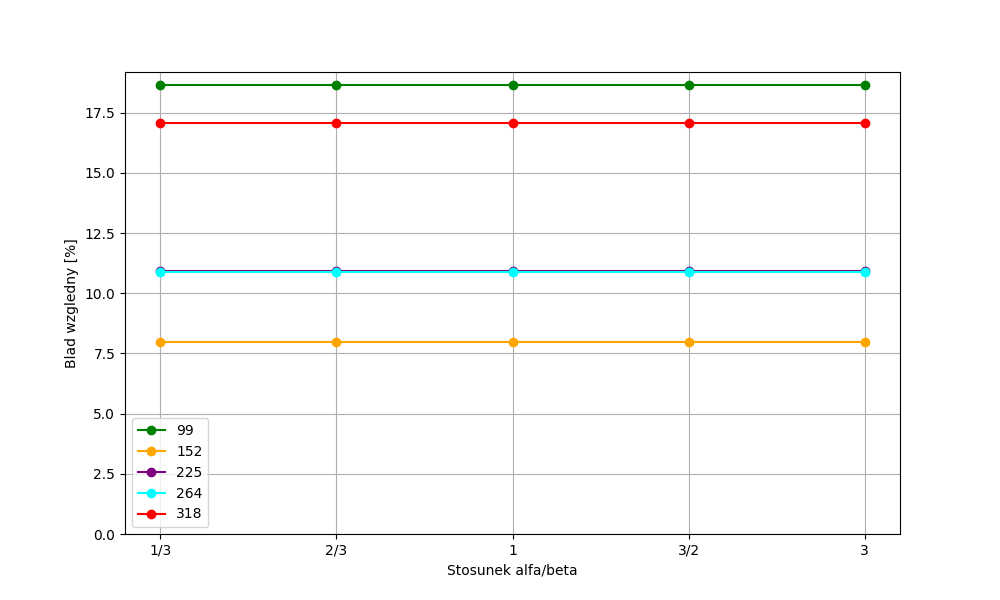
\includegraphics[width=\textwidth]{src/plots/symAoAB.png}
          \caption{Wyniki badań dla macierzy symetrycznych}
          \label{fig:symAB}
        \end{figure}
        \begin{figure}[ht]
          \centering
          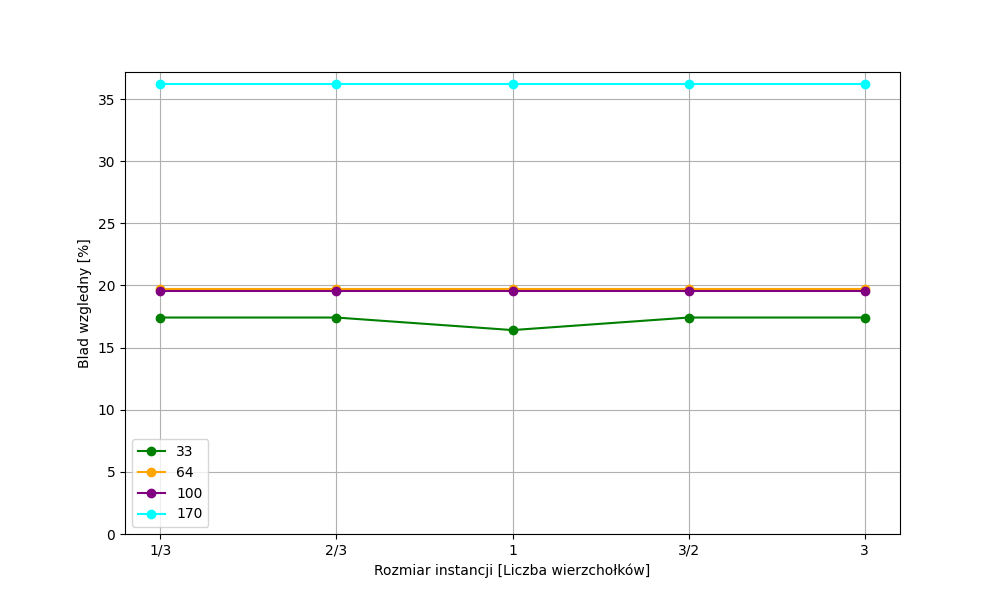
\includegraphics[width=\textwidth]{src/plots/asymAoAB.png}
          \caption{Wyniki badań dla macierzy asymetrycznych}
          \label{fig:asymAB}
        \end{figure}
        \FloatBarrier
        \begin{table}
\centering
\begin{tabular}{|r|r|r|r|r|r|r|r|r|r|r|}
\hline
 & \multicolumn{6}{|c|}{Symetryczne} & \multicolumn{4}{|c|}{Asymetryczne} \\ \hline\
Rozmiar & 99 & 152 & 225 & 264 & 318 & 439 & 33 & 64 & 100 & 170 \\ \hline
1/3 & 0.009 & 0.048 & 0.221 & 0.411 & 0.846 & 3.006 & 0.000 & 0.002 & 0.010 & 0.074 \\
2/3 & 0.009 & 0.049 & 0.222 & 0.414 & 0.855 & 3.037 & 0.000 & 0.002 & 0.010 & 0.077 \\
1 & 0.010 & 0.049 & 0.222 & 0.414 & 0.856 & 3.038 & 0.000 & 0.002 & 0.010 & 0.075 \\
3/2 & 0.010 & 0.049 & 0.222 & 0.414 & 0.865 & 3.024 & 0.000 & 0.002 & 0.010 & 0.075 \\
3 & 0.009 & 0.048 & 0.219 & 0.410 & 0.844 & 3.019 & 0.000 & 0.002 & 0.010 & 0.075 \\ \hline
\end{tabular}
\caption{Czas znalezienia wyniku algorytmu dla macierzy symetrycznych i niesymetrycznych[s]}
\label{tab:time_AoAB}
\end{table}

        \FloatBarrier
        \begin{figure}[ht]
          \centering
          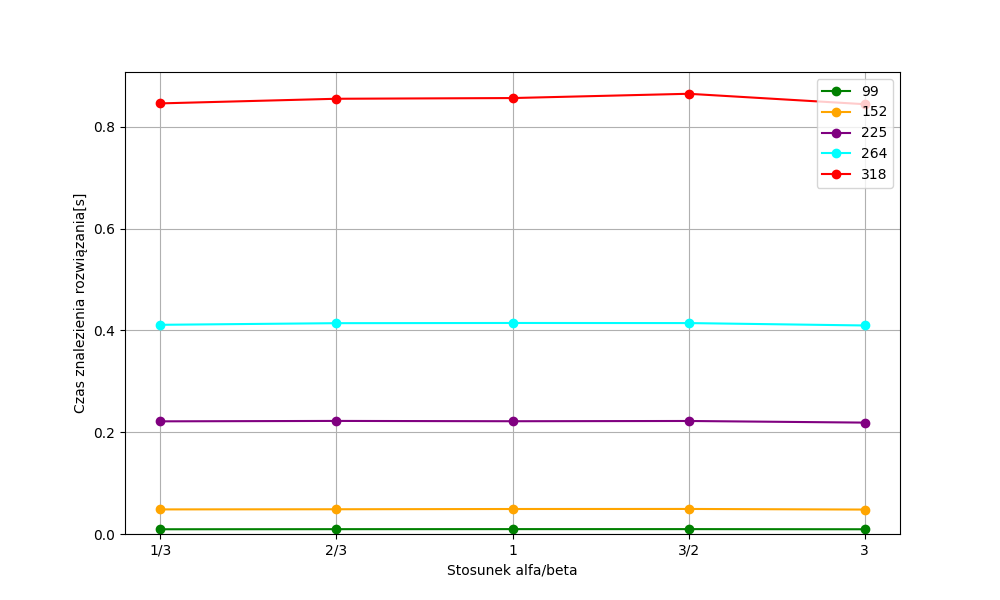
\includegraphics[width=\textwidth]{src/plots/symAoABTime.png}
          \caption{Wyniki badań dla macierzy symetrycznych}
          \label{fig:symABT}
        \end{figure}
        \begin{figure}[ht]
          \centering
          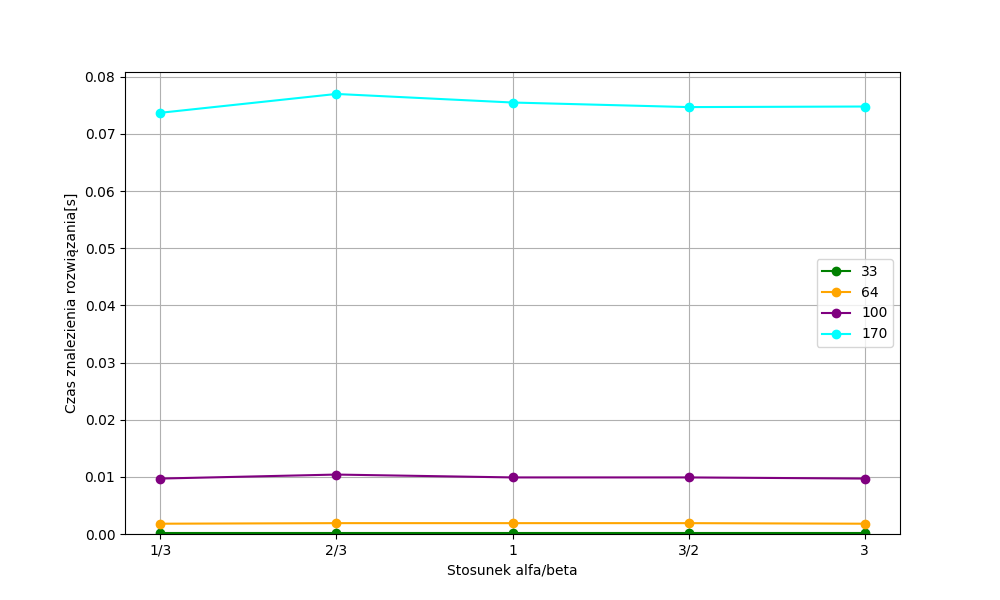
\includegraphics[width=\textwidth]{src/plots/asymAoABTime.png}
          \caption{Wyniki badań dla macierzy asymetrycznych}
          \label{fig:asymABT}
        \end{figure}
        \FloatBarrier
        \textbf{Wnioski: } Podobnie jak w przypadku badania 5.4 nie ma większych różnic
        dla różnych stosunków alfy do bety. Możliwe że podczas implementacji wzoru 
        popełniłem błąd. Możliwe też że prawdopodobieństwo wyboru nie działa poprawnie.
        Podczas testów miałem z tym wiele problemów, obene rozwiązanie działa ale może mieć problemy.
      \subsection{Podsumowanie}
        Zaimplementowany algorytm wydaje się działać poprawnie ale występuje sporo problemów. 
    \section{Wnioski z całego projektu}
      Poniżej przeprowadzono badanie dla małych tablic wykożystanych w poprzednim etapie. Dla 
      algorytmu mrówkowego podano jedynie wartości przybliżone ponieważ algorytm wykonywał się
      zbyt szybko.  
      \begin{table}
\centering
\begin{tabular}{|r|r|r|r|r|r|r|r|r|r|r|}
\hline
 & \multicolumn{5}{|c|}{Symetryczne} & \multicolumn{4}{|c|}{Asymetryczne} \\ \hline\
Rozmiar & 8 & 9 & 10 & 11 & 12 & 8 & 9 & 10 & 11 \\ \hline
& 0.500 & 0.001 & 0.001 & 0.500 & 0.500 & 0.000 & 0.000 & 0.001 & 0.500 \\ \hline
\end{tabular}
\caption{Czas znalezienia wyniku algorytmu dla macierzy symetrycznych i niesymetrycznych[s]}
\label{tab:time_PrevTS}
\end{table}

      \FloatBarrier
      \begin{table}
\centering
\begin{tabular}{|r|r|r|r|r|r|r|r|r|r|r|}
\hline
 & \multicolumn{5}{|c|}{Symetryczne} & \multicolumn{4}{|c|}{Asymetryczne} \\ \hline\
Rozmiar & 8 & 9 & 10 & 11 & 12 & 8 & 9 & 10 & 11 \\ \hline
 & 0.002 & 0.013 & 0.014 & 0.014 & 0.014 & 0.001 & 0.013 & 0.007 & 0.014 \\ \hline
\end{tabular}
\caption{Czas znalezienia wyniku algorytmu dla macierzy symetrycznych i niesymetrycznych[s]}
\label{tab:time_PrevAn}
\end{table}

      \FloatBarrier
      \begin{table}
\centering
\begin{tabular}{|r|r|r|r|r|r|r|r|r|r|r|}
\hline
 & \multicolumn{5}{|c|}{Symetryczne} & \multicolumn{4}{|c|}{Asymetryczne} \\ \hline\
Rozmiar & 8 & 9 & 10 & 11 & 12 & 8 & 9 & 10 & 11 \\ \hline
& 0.001 & 0.001 & 0.001 & 0.001 & 0.001 & 0.001 & 0.001 & 0.001 & 0.001 \\\hline
\end{tabular}
\caption{Czas znalezienia wyniku algorytmu dla macierzy symetrycznych i niesymetrycznych[s]}
\label{tab:time_PrevAo}
\end{table}

      \FloatBarrier
    \section{Źródła}
      \begin{enumerate}[label=\arabic*.]
        \item \url{https://www.javatpoint.com/what-is-a-tabu-search}
        \item \url{https://www.geeksforgeeks.org/what-is-tabu-search/}
        \item \url{https://www.baeldung.com/cs/tabu-search}
        \item \url{http://comopt.ifi.uni-heidelberg.de/software/TSPLIB95/} \label{src:TspLib}
        \item \url{https://eportal.pwr.edu.pl/pluginfile.php/209250/mod_resource/content/1/w8.pdf}
        \item \url{https://www.geeksforgeeks.org/introduction-to-ant-colony-optimization/}
      \end{enumerate}
\end{document}